\documentclass{article}

\def\npart{III}
\def\nyear{2018}
\def\nterm{Michaelmas}
\def\nlecturer{Dr. P. Varj\'{u}}
\def\ncourse{Topics in Ergodic Theory}
\def\draft{Ongoing course, rough}

% preamble
\usepackage{imakeidx}
\usepackage{marginnote}

\ifx \nauthor\undefined
  \def\nauthor{Bhavik Mehta}
\else
\fi

\author{Based on lectures by \nlecturer \\\small Notes taken by \nauthor}
\date{\nterm\ \nyear}
\title{Part \npart\ -- \ncourse}

\usepackage[utf8]{inputenc}
\usepackage{amsmath}
\usepackage{amsthm}
\usepackage{amssymb}
\usepackage{enumerate}
\usepackage{mathtools}
\usepackage{graphicx}
\usepackage[dvipsnames]{xcolor}
\usepackage{tikz}
\usepackage{wrapfig}
\usepackage{centernot}
\usepackage{float}
\usepackage{braket}
\usepackage[hypcap=true]{caption}
\usepackage{enumitem}
\usepackage[colorlinks=true, linkcolor=mblue]{hyperref}
\usepackage[nameinlink,noabbrev]{cleveref}
\usepackage{nameref}
\usepackage[margin=1.5in]{geometry}

% Theorems
\theoremstyle{definition}
\newtheorem*{aim}{Aim}
\newtheorem*{axiom}{Axiom}
\newtheorem*{claim}{Claim}
\newtheorem*{cor}{Corollary}
\newtheorem*{conjecture}{Conjecture}
\newtheorem*{defi}{Definition}
\newtheorem*{eg}{Example}
\newtheorem*{ex}{Exercise}
\newtheorem*{fact}{Fact}
\newtheorem*{law}{Law}
\newtheorem*{lemma}{Lemma}
\newtheorem*{notation}{Notation}
\newtheorem*{prop}{Proposition}
\newtheorem*{question}{Question}
\newtheorem*{rrule}{Rule}
\newtheorem*{thm}{Theorem}
\newtheorem*{assumption}{Assumption}

\newtheorem*{remark}{Remark}
\newtheorem*{warning}{Warning}
\newtheorem*{exercise}{Exercise}

% \newcommand{\nthmautorefname}{Theorem}

\newtheorem{nthm}{Theorem}[section]
\newtheorem{nlemma}[nthm]{Lemma}
\newtheorem{nprop}[nthm]{Proposition}
\newtheorem{ncor}[nthm]{Corollary}
\newtheorem{ndef}[nthm]{Definition}

% Special sets
\newcommand{\C}{\mathbb{C}}
\newcommand{\N}{\mathbb{N}}
\newcommand{\Q}{\mathbb{Q}}
\newcommand{\R}{\mathbb{R}}
\newcommand{\Z}{\mathbb{Z}}

\newcommand{\abs}[1]{\left\lvert #1\right\rvert}
\newcommand{\norm}[1]{\left\lVert #1\right\rVert}
\renewcommand{\vec}[1]{\boldsymbol{\mathbf{#1}}}

\let\Im\relax
\let\Re\relax

\DeclareMathOperator{\Im}{Im}
\DeclareMathOperator{\Re}{Re}
\DeclareMathOperator{\id}{id}

\definecolor{mblue}{rgb}{0., 0.05, 0.6}

\makeindex[intoc]
\reversemarginpar

\newcommand{\named}[1]{\textbf{#1}\index{#1}}

\DeclareMathOperator*{\dlim}{D-lim}
\DeclareMathOperator*{\clim}{C-lim}
\DeclareMathOperator*{\limw}{lim-w}

\newcommand{\B}{\mathcal{B}}
\newcommand{\sym}{\bigtriangleup}

% and here we go!

\begin{document}
\maketitle

\tableofcontents

\clearpage
% lecture 1
\section{Measure preserving systems}
Ergodic \marginnote{\emph{Lecture 1}}theory is all about measure preserving systems.
\begin{defi}[Measure preserving system]\index{measure preserving!system}\hypertarget{def:mps}
  A \textbf{measure preserving system} $(X, \mathcal{B}, \mu, T)$ with $X$ a set, $\mathcal{B}$ a $\sigma$-algebra, $\mu$ a probability measure ($\mu(A) \geq 0$ $\forall A \in \mathcal{B}$ and $\mu(X) = 1$) and $T$ is a measure preserving transformation.
  \index{measure preserving!transformation}Recall a \textbf{measure preserving transformation} $T : X \to X$ is a measurable function such that $\mu(T^{-1}(A)) = \mu(A)$ $\forall A \in \mathcal{B}$.
\end{defi}
If $Y$ is a random element of $X$ with distribution $\mu$, then $T(Y)$ also has distribution $\mu$.

\begin{eg}
  \index{circle rotation map}\hypertarget{def:circ}For example, consider a circle rotation. We have $X = \mathbb{R}/\mathbb{Z}$, $\mathcal{B}$ is the Borel sets, $\mu$ the Lebesgue measure, and $T = R_\alpha$, with $x \mapsto x + \alpha$ and $\alpha \in \mathbb{R}/\mathbb{Z}$ is a parameter.

  \index{doubling map}\hypertarget{def:doubling}We also have the `times 2' or `doubling' map, with the same $X, \mathcal{B}, \mu$ and $T = T_2$, $x \mapsto 2 \cdot x$.
\end{eg}
\begin{proof}[Proof that \hyperlink{def:doubling}{$T_2$} is \hyperlink{def:mps}{measure preserving}]
  First check for intervals: Let $I = (a,b)$, then $\mu(I) = b-a$.
  Also, $\mu(T_2^{-1}I) = \mu\left((\frac{a}{2},\frac{b}{2}) \cup (\frac{a}{2} + \frac{1}{2}, \frac{b}{2} + \frac{1}{2})\right) = \frac{b}{2} - \frac{a}{2} + \frac{b}{2} - \frac{a}{2} = b - a$, as required.

  Now, let $U \subset \mathbb{R}/\mathbb{Z}$ be open. Then $U = I_1 \sqcup I_2 \sqcup \dotsb$ is a disjoint union of intervals:
  \begin{align*}
    \mu(T^{-1} U) &= \mu\left(\bigcup T^{-1} I_j\right) \\
                  &= \sum \mu(T^{-1} I_j) \\
                  &= \sum \mu(I_j) \\
                  &= \mu(U).
  \end{align*}
  Let $K \subset \mathbb{R}/\mathbb{Z}$ be a compact set.
  \begin{align*}
    \mu(T^{-1} K) = 1 - \mu((T^{-1} K)^c) = 1 - \mu(T^{-1} K^c) = 1 - \mu(K^c) = \mu(K).
  \end{align*}
  Now let $A \in \mathcal{B}$ be arbitrary. Let $\epsilon > 0$. $\exists U$ open and $\exists K$ compact such that $K \subset A \subset U$ and $\mu(U \setminus K) < \epsilon$.
  \begin{align*}
    \mu(K) = \mu(T^{-1} K) \leq \mu(T^{-1} A) \leq \mu(T^{-1} U) = \mu(U).
  \end{align*}
  We also have $\mu(K) \leq \mu(A) \leq \mu(U)$.
  Since $\mu(U) - \mu(K) < \epsilon$, $|\mu(A) - \mu(T^{-1}A)| < \epsilon$. $\epsilon$ was arbitrary, so $\mu(A) = \mu(T^{-1} A)$.
\end{proof}

The two examples generalise to the Haar measure on a topological group and to endomorphisms respectively.

In ergodic theory, we study the long term behaviour of orbits.
\begin{defi}[Orbit]\index{orbit}\hypertarget{def:orbit}
  The orbit of $x \in X$ is the sequence
  \begin{equation*}
    x, Tx, T^2 x, \dotsc
  \end{equation*}
\end{defi}
Some questions we might ask are:
\begin{itemize}
  \item Let $A \in \mathcal{B}$ and $x \in A$.
    Does the \hyperlink{def:orbit}{orbit} of $x$ visit $A$ infinitely often? (Recurrence)
  \item What is the proportion of times $n$ such that $T^n x \in A$? (Ergodicity)
  \item What is $\mu(\set{x \in A | T^n x \in A})$ if $n$ is large? (Mixing)
\end{itemize}

\begin{eg}
  Let $A = [0, \frac{1}{4}) \subset \mathbb{R}/\mathbb{Z}$. %]
  Then $\hyperlink{def:doubling}{T_2^n} x \in A \iff $ the $n+1$th and $n+2$th `binary digits' of $x$ are $0$:

  For $x = 0.x_1 x_2 x_3 \dots_2$, $x \in A$ corresponds to $x_1, x_2$ both being 0 and the \hyperlink{def:doubling}{doubling map} sends $x$ to $T_2x = x_2 x_3 \dots_2$, showing the required property.

  For example, $x = \frac{1}{6} = 0.00101010\dots_2$ starts in $A$ but never comes back to $A$, but `most points' do return to $A$.
  Also, we have $\mu(\set{x \in A | T_2^n x}) = \frac{1}{16}$ for any $n \geq 2$.
\end{eg}

\begin{eg}[Markov shift]\index{Markov shift}\hypertarget{def:markovshift}
  Let $(P_1, P_2, \dotsc, P_n)$ be a probability vector.
  Let $A \in \mathbb{R}^{n \times n}_{\geq 0}$ be the `matrix of transition probabilities'.
  Assume
  \begin{equation*}
    A
    \begin{pmatrix}
      1 \\ 1 \\ \vdots \\ 1
    \end{pmatrix}
    =
    \begin{pmatrix}
      1 \\ 1 \\ \vdots \\ 1
    \end{pmatrix}, \quad
    \begin{pmatrix}
      P_1 & P_2 & \dots & P_n
    \end{pmatrix}
    A =
    \begin{pmatrix}
      P_1 & P_2 & \dots & P_n
    \end{pmatrix}
  \end{equation*}
  Take $X = \{1, \dotsc, n\}^\mathbb{Z}$, $\mathcal{B} =$ Borel $\sigma$-algebra generated by the product topology of the discrete topology on $\{1, \dotsc, n\}$, $T = \sigma$ the shift map: $(\sigma x)_m = x_{m+1}$.
  Finally, set the measure
  \begin{equation*}
    \mu(\set{x \in X | x_m = i_0, x_{m+1} = i_1, \dotsc, x_{m+n} = i_n}) = P_{i_0} a_{i_0 i_1} \dotsm a_{i_{n-1} i_n}.
  \end{equation*}
  On the example sheet, we will confirm this extends to a measure and that it is invariant under $T$.
\end{eg}

\clearpage
\section{Furstenberg correspondence}
An interesting problem from number theory and combinatorics is Szemer\'edi's theorem.
In this course, we will give an ergodic theory proof of this, using Furstenberg's multiple recurrence theorem.
\begin{thm}[Szemer\'{e}di's theorem]\index{Szemer\'{e}rdi's theorem}\hypertarget{thm:sze}
  Let $S \subset \mathbb{Z}$ of positive upper Banach density. That is,
  \begin{equation*}
    \bar{d}(S) \coloneqq \limsup_{N,M: M - N \to \infty} \frac{1}{M-N} \big| S \cap [N,M-1] \big|
  \end{equation*}
  and $\bar{d}(S) > 0$.
  Then $S$ contains arbitrarily long arithmetic progressions. That is, $\forall l, \exists a \in \mathbb{Z}, d \in \mathbb{Z}_{> 0}$,
  \begin{equation*}a, a+d, \dotsc, a+(l-1)d \in S.\end{equation*}
\end{thm}

\begin{thm}[Furstenberg, multiple recurrence]\index{Furstenberg multiple recurrence}\hypertarget{thm:furs}
  Let $(X, \mathcal{B}, \mu, T)$ be a \hyperlink{def:mps}{measure preserving system}. Let $A \in \mathcal{B}$ such that $\mu(A) > 0$. Let $l \in \mathbb{Z}_{>0}$.
  Then
  \begin{equation*}
    \liminf_{N \to \infty} \frac{1}{N} \sum_{n=1}^N \mu(A \cap T^{-n} A \cap \dotsb \cap T^{-(l-1) n} A) > 0.
  \end{equation*}
\end{thm}

% lecture 2
To \marginnote{\emph{Lecture 2}}prove \hyperlink{thm:furs}{Furstenberg's theorem} requires more preparation, and we will do it later in this course.
However, we can now prove \hyperlink{thm:sze}{Szemer\'edi} assuming \hyperlink{thm:furs}{Furstenberg multiple recurrence}.

\begin{proof}[Proof of \hyperlink{thm:sze}{Szemer\'edi} using \hyperlink{thm:furs}{Furstenberg}]
  Aim to construct a \hyperlink{def:mps}{measure preserving system} in order to use \hyperlink{thm:furs}{Furstenberg multiple recurrence}, using the given set $S$.

  Take $X = \{0, 1\}^\Z$, $\mathcal{B}=$ Borel $\sigma$-algebra and
  $\sigma=$ the \hyperlink{def:markovshift}{shift} map $(\sigma(x))_n = x_{n+1}$.
  Let $ {x}^S \in X$ be defined by
  \begin{equation*}
    {x}_n^S =
    \begin{cases}
      1 & n\in S\\
      0 & n \notin S
    \end{cases}
  \end{equation*}
  (so $x^S$ is effectively the indicator function of $S$).
  Also let $A\in\mathcal{B}$ be given by $A = \set{{x}\in X | x_0 = 1}$.
  Observe then that
  \begin{equation*}
    n\in S\iff x^S_n=1\iff (\sigma^n x^S)_0=1\iff \sigma^n x^S\in A.
  \end{equation*}
  The equivalence $n \in S \iff \sigma^n x^S \in A$ allows us to relate the set $S$ to the dynamics of $\sigma$.

  Now, we begin to construct the invariant measure $\mu$.
  Let $\{M_m\}$ and $\{N_m\}$ be sequences s.t. $ M_n-N_m\to\infty $ and
  \begin{equation*} \bar{d}(S) = \lim_{m\to\infty}\frac{1}{M_m-N_m}\left|S\cap[N_m,M_m-1]\right|. \end{equation*}
  Let
  \begin{equation*}
    \mu_m = \frac{1}{M_m-N_m}\sum_{n=N_m}^{M_m-1}\delta_{\sigma^n{x}^S}
  \end{equation*}
  where $\delta_x$ is a measure on $X$ defined as
  \begin{equation*}
    \delta_x(B) =
    \begin{cases}
      1 & x\in B\\
      0 & x\notin B.
    \end{cases}
  \end{equation*}

  Let $\mu$ be the \hyperlink{def:weaklimit}{weak limit} of \emph{a} subsequence of $\mu_m$.
  Note that the $\mu$ could be different dependent on subsequence choice.
  \renewcommand{\qedsymbol}{}
\end{proof}

\subsection{Aside on weak limits}
We pause the proof to briefly recap material on weak limits.

\begin{defi}[Weak limit]\hypertarget{def:weaklimit}
  Let $X$ be a compact metric space.
  Let $\mu_m$ be a sequence of Borel measures on $X$, and let $\mu$ be another Borel measure.
  \index{weak limit}Then $\mu_m$ \textbf{converges weakly} to $\mu$ if for any $f\in C(X)$, we have
  \begin{equation*}
    \lim _{n \to \infty} \int_X f \,d \mu_{n} = \int_X f \,d \mu.
  \end{equation*}
  We write $\limw_{n \to \infty} \mu_n = \mu$.
\end{defi}

\begin{thm}[Banach-Alaoglu, or Helly]\hypertarget{thm:banachalaoglu}
  Let $X$ be a compact metric space.
  \index{Banach-Alaoglu theorem}Then $\mathcal{M}(X)$, the set of Borel probability measures on $X$, endowed with the topology of weak convergence, is compact and metrizable.
  That is, there is a \hyperlink{def:weaklimit}{weakly convergent subsequence} in any sequence of Borel probability measures.
\end{thm}

We are ready to return to the main proof: next we check that the system constructed is indeed a \hyperlink{def:mps}{measure preserving system}.
\begin{lemma}
  $(X, \mathcal{B}, \mu, \sigma)$ as defined above is a \hyperlink{def:mps}{measure preserving system}.
\end{lemma}
\begin{proof}[Proof sketch]
  Let $B \in \mathcal{B}$. Then
  \begin{align*}
    \mu_m(B) &= \frac{1}{M_m - N_m} \left\lvert\set{n \in [N_m, M_m -1] | \sigma^n {x}^S \in B} \right\rvert \\
    \mu_m(\sigma^{-1} B) &= \frac{1}{M_m - N_m} \left|\set{n \in [N_m, M_m -1] | \sigma^n {x}^S \in \sigma^{-1}B} \right| \\
                         &= \frac{1}{M_m - N_m} \left|\set{n \in [N_m+1, M_m] | \sigma^n {x}^S \in B} \right|
  \end{align*}
  So the difference is such that
  \begin{equation*} \left|\mu_m(B) - \mu_m(\sigma^{-1}B)\right| \leq \frac{1}{M_m-N_m}\to 0 \end{equation*}
  It can be shown that we can pass to the limit on $m$ and conclude that $\mu(B) = \mu(\sigma^{-1}B)$.
\end{proof}

\begin{remark}
  If $B$ is a cylinder set, i.e.\ $\exists L \in \mathbb{Z}_{>0}$ and $\tilde{B} \subseteq \{0,1\}^{2L+1}$ such that
  \begin{equation*}
    B = \set{x \in X | (x_{-L}, \dotsc, x_L) \in \tilde{B}},
  \end{equation*}
  then $B$ is both closed and open.
  Therefore $\chi_B$, the characteristic function of $B$ is continuous.
  Hence $\lim_{n \to \infty} \mu_m(B) = \mu(B)$, since $\mu_m(B) = \int \chi_B \, d \mu_m$ and $\mu(B) = \int \chi_B \, d \mu$.

  Approximating any Borel set by such cylinder sets would help complete the proof, but we in fact can get this result on spaces where $\chi$ is not continuous on a nice set of sets.
  So we leave full proof till a more general theorem.
\end{remark}

\begin{prop}
  Let $S \subseteq \mathbb{Z}$, $x^S, A, (X, \mathcal{B}, \mu, \sigma)$ as defined above.
  Let $l \in \mathbb{Z}_{> 0}$.
  Suppose that $\exists n \in \mathbb{Z}_{>0}$ such that
  \begin{equation*}
    \mu\left(A \cap \sigma^{-n}(A) \cap \dotsb \cap \sigma^{-n(l-1)}(A)\right) > 0.
  \end{equation*}
  Then $S$ contains an arithmetic progression of length $l$.
\end{prop}
\begin{proof}
  Without loss of generality, we can assume $\mu = \hyperlink{def:weaklimit}{\limw} \mu_m$ - if not, pass to a subsequence.
  Let $B = A \cap \sigma^{-n} A \cap \dotsb \cap \sigma^{-n (l-1)} (A).$
  Observe that $B$ is a cylinder set.
  Then by the remark, $\mu(B) = \lim \mu_m(B)$, hence $\exists m$ such that $\mu_m(B) > 0$.

  By definition of $\mu_m$, $\exists k \in [N_m, M_m - 1]$ such that $\sigma^k x^S \in B$.
  Hence
  \begin{equation*}\sigma^k x^S \in A, \sigma^k x^S \in \sigma^{-n}(A), \dotsc, \sigma^k x^S \in \sigma^{-n(l-1)}(A).\end{equation*}
  Thus, $k, k+n, \dotsc, k + n(l-1) \in S$.
\end{proof}
Returning to the overall proof, we note $A$ is a cylinder set.
Then $ \mu_m(A)\to\mu(A) $, i.e.\
\begin{equation*} \mu(A) = \underbrace{\lim_{m\to\infty}\frac{1}{M_m-N_m}\left|\set{n\in[N_m,M_m-1]: n\in S}\right|}_{\bar{d}(S)} > 0 \end{equation*}
where the inequality comes from satisfying the conditions of \hyperlink{thm:sze}{Szemer\'edi}, and \hyperlink{thm:furs}{Furstenberg's multiple recurrence} finishes the argument. \qed

\clearpage
\section{Ergodicity}
\begin{lemma}
  \marginnote{\emph{Lecture 3}}Let $(X, \mathcal{B}, \mu, T)$ be a \hyperlink{def:mps}{measure preserving system}.
  Let $A \in \mathcal{B}$ with $\mu(A) > 0$. Then $\exists n \in \mathbb{Z}_{> 0}$ such that $\mu(A \cap T^{-n} A) > 0$.
\end{lemma}
\begin{proof}
  Suppose for contradiction that $\mu(A \cap T^{-n}A) = 0$ for all $n > 0$.
  Then
  \begin{equation*}\mu(T^{-k}A \cap T^{-n} A) = \mu(A \cap T^{-(n-k)}A) = 0\end{equation*}
  for all $n > k \geq 0$.
  Thus the sets $A, T^{-1} A, \dotsc$ are `almost pairwise disjoint'.

  Then
  \begin{align*}
    \mu(A \cup T^{-1} A \cup \dotsb \cup T^{-n} A) &= \mu(A) \\
                                                   &+ \mu(T^{-1} A) - \underbrace{\mu(T^{-1}A \cap A)}_{=0} \\
                                                   &+ \mu(T^{-2} A) - \underbrace{\mu(T^{-2} A \cap (A \cup T^{-1} A))}_{=0} \\
                                                   &\vdotswithin{-}\\
                                                   &+ \mu(T^{-n} A) - \underbrace{\mu(T^{-n} A \cap (A \cup T^{-1} A \cup \dotsb \cup T^{-(n-1)} A))}_{=0} \\
                                                   &= (n+1) \mu(A),
  \end{align*}
  a contradiction if $n + 1 > \mu(A)^{-1}$.
\end{proof}
\begin{thm}[Poincar\'{e} recurrence]\hypertarget{thm:poincare}
  Let $(X, \mathcal{B}, \mu, T)$ be a \hyperlink{def:mps}{measure preserving system}.
  \index{Poincar\'e recurrence}Let $A \in \mathcal{B}$ with $\mu(A) > 0$.
  Then almost every $x \in A$ returns to $A$ infinitely often.
  That is:
  \begin{equation*}
    \mu\left(A \setminus \bigcap_{N=1}^\infty \bigcup_{n=N}^\infty T^{-n} A\right) = 0.
  \end{equation*}
\end{thm}
\begin{remark}
  $x \in T^{-n} A \iff T^n x \in A$. $\bigcup_{n=N}^\infty T^{-n} A$ are the points that visit $A$ at least once after time $N$.
\end{remark}
\begin{proof}
  Let $A_0$ be the set of points in $A$ that never return to $A$.
  We first show $\mu(A_0) = 0$.
  Note that
  \begin{equation*}\mu(A_0 \cap T^{-n} A_0) \leq \mu(A_0 \cap T^{-n} A) = \mu(\emptyset) = 0\end{equation*}
  for all $n > 0$.
  By the lemma, $\mu(A_0) = 0$.

  Note that if
  \begin{equation*}x \in A \setminus \bigcap_{N=1}^\infty \bigcup_{n=N}^\infty T^{-n} A,\end{equation*}
  then there is a maximal $m \in \mathbb{Z}_{\geq 0}$ such that $T^m x \in A_0$.
  This means that
  \begin{equation*}
    A \setminus \bigcap \bigcup T^{-n} A \subset \bigcup_{m=0}^\infty T^{-m} A_0
  \end{equation*}
  where the right hand side has measure 0.
\end{proof}

This effectively answers the first question we asked earlier - the \hyperlink{def:orbit}{orbit} of almost every $x$ visits $A$ infinitely often if $\mu(A) > 0$.

But what if the point does not start in $A$?
The main issue that can occur is that $X$ splits into parts, which are preserved under $T$:
\begin{center}
  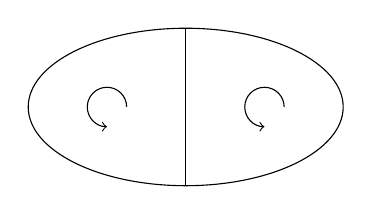
\begin{tikzpicture}
    \draw (0,0) circle[x radius=2cm, y radius=1cm];
    \draw (0,-1) -- (0,1);
    \draw [->] (-0.75,0) arc[radius=2.5mm, start angle= 0, end angle= 270];
    \draw [->] (1.25,0) arc[radius=2.5mm, start angle= 0, end angle= 270];
  \end{tikzpicture}
\end{center}

So, we define a notion of `irreducible' for \hyperlink{def:mps}{measure preserving systems}.
\begin{defi}[Ergodic]\hypertarget{def:ergodic}
  A \hyperlink{def:mps}{measure preserving system} is called \named{ergodic} if $A = T^{-1}A$ implies $\mu(A) = 0$ or $1$ for all $A \in \mathcal{B}$.
\end{defi}

If a \hyperlink{def:mps}{measure preserving system} is not \hyperlink{def:ergodic}{ergodic}, we have $A \in \mathcal{B}$ with $0 < \mu(A) < 1$ such that $T^{-1} A = A$, then we can restrict the measure preserving system to $A$.
That is, we consider the measure preserving system $(A, \mathcal{B}_A, \mu_A, T|_A)$ where $\mathcal{B}_A = \set{B \in \mathcal{B} | B \subseteq A}$ and $\mu_A(B) = \frac{\mu(B)}{\mu(A)}$ for all $B \in \mathcal{B}_A$.
\begin{thm}
  The following are equivalent for an \hyperlink{def:mps}{measure preserving system} $(X, \mathcal{B}, \mu,T)$.
  \begin{enumerate}[label=(\arabic*)]
    \item $(X, \mathcal{B}, \mu, T)$ is \hyperlink{def:ergodic}{ergodic}.
    \item For all $A \in \mathcal{B}$ with $\mu(A) > 0$,
      \begin{equation*}
        \mu\left(\bigcap_{N=1}^\infty \bigcup_{n=N}^\infty T^{-n} A\right) = 1.
      \end{equation*}
    \item $\mu(A \sym T^{-1} A) = 0$ implies $\mu(A) = 0$ or $1$ $\forall A \in \mathcal{B}$.
    \item For all bounded measurable functions $f: X \to \mathbb{R}$,
      $f = f \circ T$ almost everywhere implies $f$ is constant almost everywhere.
    \item For all bounded measurable functions $f: X \to \mathbb{C}$,
      $f = f \circ T$ almost everywhere implies $f$ is constant almost everywhere.
  \end{enumerate}
\end{thm}
\begin{proof}
  (1) $\Rightarrow$ (2).
  Let $A \in \mathcal{B}$ with $\mu(A) > 0$. Let $B = \bigcap \bigcup T^{-n}A$.
  By \hyperlink{thm:poincare}{Poincar\'e recurrence}, $\mu(B) \geq \mu(A) > 0$.
  So if we show that $B = T^{-1} B$, then $\mu(B) = 1$ follows by \hyperlink{def:ergodic}{ergodicity}.
  But
  \begin{equation*}x \in B \iff x\text{ visits }A\text{ infinitely often }\iff Tx\text{ visits }A\text{ infinitely often }\iff Tx \in B.\end{equation*}
  So $B = T^{-1} B$.

  (2) $\Rightarrow$ (3). Let $A \in \mathcal{B}$ such that $\mu(A \sym T^{-1} A) = 0$. If $\mu(A) = 0$, there is nothing to prove. Suppose $\mu(A) > 0$.
  Let $B = \bigcap \bigcup T^{-n} A$. By (2), we know that $\mu(B) = 1$.

  We show $\mu(B \setminus A) = 0$, which completes the proof.
  Let $x \in B \setminus A$, then there is a first time $m$ such that $T^m x \in A$, and $m > 0$.
  Hence $x \in T^{-m} A \setminus T^{-(m-1)}A$. Thus
  \begin{equation*}
    B \setminus A \subseteq \bigcup_m T^{-m} A \setminus T^{-(m-1)} A,
  \end{equation*}
  and $\mu(T^{-m} A \setminus T^{-(m-1)} A) = \mu(T^{-1} A \setminus A) = 0$, so $\mu(B \setminus A) = 0$.

  (3) $\Rightarrow$ (4).
  Let $f : X \to \mathbb{R}$ be a bounded measurable function such that $f = f \circ T$ almost everywhere.
  For all $t \in \mathbb{R}$, let $A_t = \set{x \in X | f(x) \leq t}$.
  Then $\mu(A_t \sym T^{-1} A_t) = 0$.
  By (3), we have $\mu(A_t) = 0$ or $1$ for all $t$.

  If $t$ is very small, then $\mu(A_t) = 0$. If $t$ is very large, $\mu(A_t) = 1$. $t \mapsto \mu(A_t)$ is monotone, hence $\exists c \in \mathbb{R}$ such that $\mu(A_t) = 0$ for all $t < c$ and $\mu(A_t) = 1$ $\forall t > c$.
  Then $f(x) = c$ almost everywhere.

  (4) $\Leftrightarrow$ (5) is left as an exercise.

  (4) $\Rightarrow$ (1). Let $A \in \mathcal{B}$ with $A = T^{-1} A$. Then $\chi_A = \chi_A \circ T$ everywhere so $\chi_A$ is constant almost everywhere.
\end{proof}
\begin{eg}
  The \hyperlink{def:circ}{circle rotation} map $(\mathbb{R}/\mathbb{Z}, \mathcal{B}, \mu, R_\alpha)$ is \hyperlink{def:ergodic}{ergodic} iff $\alpha$ is irrational.
  Let $f: X \to \mathbb{R}$ be measurable. We can write $f(x) = \sum_{n \in \mathbb{Z}} a_n \exp(2\pi i n x)$.
  \begin{align*}
    f \circ R_\alpha(x) = f(x + \alpha) &= \sum_{n \in \mathbb{Z}} a_n \exp(2 \pi i n (x + \alpha)) \\
                                        &= \sum_{n \in \mathbb{Z}} a_n \exp(2\pi i n \alpha) \exp(2 \pi i n x)
  \end{align*}
  So $f = f \circ R_\alpha \iff a_n = a_n \exp(2 \pi i n \alpha) \; \forall n$. If $\alpha$ is irrational, then $\exp(2 \pi i n \alpha) \neq 1$ for all $n \neq 0$, so $a_n = 0$.
\end{eg}

% lecture 4
\clearpage
\section{Ergodic theorems}
In \marginnote{\emph{Lecture 4}}the previous section, we discussed recurrence, which is concerned with orbits visiting a particular set infinitely often.
However, we have not addressed how frequent these visits are: the second question we asked earlier.
\begin{thm}[Mean Ergodic Theorem, von Neumann]\index{ergodic theorem!mean}\index{mean ergodic theorem}\hypertarget{thm:meanet}
  Let $(X, \mathcal{B}, \mu, T)$ be a \hyperlink{def:mps}{measure preserving system}, and write
  \begin{equation*}
    \hypertarget{def:invfunc}I \coloneqq \set{f \in L^2(X) | f \circ T = f \text{ a.e.}}
  \end{equation*}
  for the (closed) subspace of $T$-invariant functions.
  Denote by $P_T:L^2(X) \to I$ the orthogonal projection.
  Then for every $f \in L^2(X)$:
  \begin{equation*}
    \frac{1}{N} \sum_{n=0}^{N-1} f \circ T^n \to P_T f \quad \text{in } L^2(X).
  \end{equation*}
\end{thm}
\begin{thm}[Pointwise Ergodic Theorem, Birkhoff]\index{ergodic theorem!pointwise}\index{pointwise ergodic theorem}\hypertarget{thm:pet}
  Let $(X, \mathcal{B}, \mu, T)$ be a \hyperlink{def:mps}{measure preserving system}.
  Then for every $f \in L^1(X)$, there is a $T$-invariant function
  $f^* \in L^1(X)$ such that
  \begin{equation*}
    \frac{1}{N} \sum_{n=0}^{N-1} f \circ T^n \to f^*(x) \quad \text{pointwise a.e.}
  \end{equation*}
\end{thm}

\hypertarget{def:ergavg}When $f \in L^2(X)$, then the function $f^*$ in the \hyperlink{thm:pet}{Pointwise Ergodic Theorem} is $P_Tf$.
The \hyperlink{thm:meanet}{Mean Ergodic Theorem} also holds in $L^p$ for $1 \leq p < \infty$, see the example sheet.
We call the quantity $\frac{1}{N} \sum_{n=0}^{N-1} f \circ T^n$ the \named{ergodic average}.

\begin{lemma}
  Let $(X, \mathcal{B}, \mu)$ be a probability space, and let $T: X \to X$ be a measurable transformation.
  Then $T$ is \hyperlink{def:mps}{measure preserving} if and only if
  \begin{equation*}
    \int_X f \circ T \, d\mu = \int_X f \, d\mu \label{eq:4star} \tag{$*$}
  \end{equation*}
  for all $f \in L^1(X)$.
\end{lemma}
\begin{proof}
  $(\Rightarrow)$. Let $A \in \mathcal{B}$ and note that $x \in T^{-1}(A)$ is equivalent to $Tx \in A$.
  Hence we can write
  \begin{equation*}
    \mu(T^{-1}(A))=\int\!\chi_{T^{-1}A}\,d\mu=\int\!\chi_A\circ T\,d\mu=\int\!\chi_A\,d\mu=\mu(A)
  \end{equation*}
  so $T$ is measure preserving.

  ($\Leftarrow$). As in ($\Rightarrow$), we can show \eqref{eq:4star} for characteristic functions.
  Then by linearity of integration, it also holds for simple functions.
  Now let $f \in L^1(X)$ be non-negative. Taking $f_1, f_2, \dotsc$ an increasing sequence of simple functions with $f = \lim f_n$ almost everywhere.
  Then $f \circ T = \lim f_n \circ T$ almost everywhere (since $T$ is measure preserving).
  Hence using the definition of integration and \eqref{eq:4star} for simple functions
  \begin{equation*}
    \int\!f\circ T\,d\mu=\lim\int\!f_n\circ T\,d\mu=\lim\int\!f_n\,d\mu=\int\!f\,d\mu.
  \end{equation*}
  Finally, a general $f \in L^1(X)$ can be written as the difference of two non-negative functions, and conclude \eqref{eq:4star} by linearity.
\end{proof}
\begin{defi}[Koopman operator]\index{Koopman operator}\hypertarget{def:koopman}
  Let $(X,\mathcal{B}, \mu, T)$ be a \hyperlink{def:mps}{measure preserving system}.
  For $f: X \to \mathbb{C}$ a measurable function, define
  \begin{equation*}
    U_T f = f \circ T
  \end{equation*}
  and call $U_T$ the \textbf{Koopman operator}.
\end{defi}
\begin{lemma}
  The \hyperlink{def:koopman}{Koopman operator $U_T$} is an isometry on the Hilbert space $L^2(X)$, i.e.
  \begin{equation*}
    \langle f, g \rangle = \langle U_T f, U_T g \rangle
  \end{equation*}
  for all $f,g \in L^2(X)$.
\end{lemma}
\begin{proof}
  Apply the previous lemma to $f \cdot \bar{g} \in L^1(X)$.
\end{proof}

\begin{defi}[Invertible]\index{invertible}\index{measure preserving!system!invertible}\hypertarget{def:inv}
  A \hyperlink{def:mps}{measure preserving system} $(X, \mathcal{B}, \mu, T)$ is said to be \textbf{invertible} if there is a measure preserving map $S: X \to X$ such that $T \circ S = S \circ T = \operatorname{id}_X$ almost everywhere.
  If such a map exists, denote it as $T^{-1}$.
\end{defi}
\begin{eg}
  The \hyperlink{def:circ}{circle rotation} is \hyperlink{def:inv}{invertible}, but the \hyperlink{def:doubling}{doubling map} is not.
\end{eg}
\begin{lemma}
  If the \hyperlink{def:mps}{measure preserving system} $(X, \mathcal{B}, \mu, T)$ is \hyperlink{def:inv}{invertible}, then \hyperlink{def:koopman}{$U_T$} is unitary on $L^2(X)$ and $U_T^* = U_{T^{-1}}$.
\end{lemma}
\begin{proof}
  We use the earlier lemma to the function $f \cdot \overline{(g \circ T^{-1})}$:
  \begin{align*}
    \langle f, \hyperlink{def:koopman}{U_{T^{-1}}} g \rangle &= \int f \cdot \overline{g \circ T^{-1}} \, d\mu \\
                                    &= \int (f \cdot \overline{(g \circ T^{-1})}) \circ T\,d\mu \\
                                    &= \int f\circ T \cdot \bar{g}\,d\mu \\
                                    &= \langle U_T f, g \rangle
  \end{align*}
  This shows that $U_T^* = U_{T^{-1}}$. Clearly $U_T U_{T^{-1}} = U_{T^{-1}} U_T = \operatorname{id}_{L^2(X)}$, so $U_T$ is unitary.
\end{proof}
The proofs we will give of the ergodic theorems rely on the idea that convergence is easy for certain special functions.

First, the \hyperlink{def:ergavg}{ergodic averages} of a $T$-invariant function $f \hyperlink{def:invfunc}{\in I}$ are equal to $f$, so they converge to $f$.
If $f = U_T g - g$ for some $g$, then the ergodic averages become telescopic sums and only the boundary terms remain, that is:
\begin{equation*}
  \frac{1}{N} \sum_{n=0}^{N-1} U_T^n(U_T g - g) = \frac{1}{N} (U_T^N g - g)
\end{equation*}
and the right hand side is easily seen to converge to $0$.
The following lemma shows that these two type of functions are enough to look at.
\begin{lemma}
  Write
  \begin{equation*}
    B \coloneqq \set{U_T g - g | g \in L^2(X)}.
  \end{equation*}
  Then $I = B^\perp$.
\end{lemma}
It is important to note that the space $B$ is not closed. So $L^2(X) = I \oplus \bar{B}$, but not every function in $L^2(X)$ is the sum of a $T$-invariant function and an element of $B$.
\begin{proof}
  We can write
  \begin{align*}
    f \in B^\perp &\iff \langle f, \hyperlink{def:koopman}{U_T} g - g \rangle = 0 \quad \forall g \in L^2(X) \\
                  &\iff \langle f, g \rangle = \langle f, U_T g \rangle = \langle U_T^* f, g \rangle \quad \forall g \in L^2(X) \\
                  &\iff f = U_T^* f.
  \end{align*}
  If the system was \hyperlink{def:inv}{invertible}, then we could finish the proof by applying $U_T = (U_T^*)^{-1}$ to both sides of the last equation.

  But, we can prove that $f = U_T f \iff f = U_T^* f$ in the general case:
  \begin{align*}
    f = U_T f &\iff \langle f - U_T f, f - U_T f \rangle = 0 \\
              &\iff\|f\|_2^2+\|U_T f\|^2_2-\langle f,U_Tf\rangle-\langle U_Tf,f\rangle=0 \\
              &\iff\|f\|_2^2+\|U_T^*\|_2^2-\langle U_T^*f,f\rangle-\langle f,U_T^*f\rangle + (\|U_Tf\|^2_2-\|U_T^*f\|_2^2) = 0 \\
              &\iff\|f-U_T^*f\|_2^2+(\|U_Tf\|_2^2-\|U_T^*f\|_2^2)=0
  \end{align*}
  Note that both terms in the left hand side of the final equation are non-negative, since $\|U_Tf\|_2=\|f\|_2$ since $U_T$ is an isometry, and $\|U_T^*f\|_2\leq\|f\|_2$ as $\|U_T^*\|=\|U_T\|=1$.

  Thus,
  \begin{equation*}
    f = U_T f \iff f = U_T^* f\text{ and }\|f\|_2 = \|U_T^*f\|_2.
  \end{equation*}
  The second statement of the right follows from the first one, hence $f = U_T f \iff f = U_T^*f$, as required.
\end{proof}
\begin{proof}[Proof of \hyperlink{thm:meanet}{Mean Ergodic Theorem}]
  Let $f \in L^2(X)$ and fix $\epsilon > 0$.
  By the lemma, we can write $f = \hyperlink{def:invfunc}{P_T} f + \hyperlink{def:koopman}{U_T} g - g + e$ for some $e, g \in L^2(X)$ such that $\|e\|_2 < \epsilon$.
  Thus
  \begin{equation*}
    \limsup_{n \to \infty} \left\|\frac{1}{N} \sum_{n=0}^{N-1} U_T^n f - P_T f\right\|_2 \leq \limsup_{n\to \infty} \left\lVert\frac{1}{N} \left(U_T^Ng - g\right) + \frac{1}{N} \sum_{n=0}^{N-1}U_T^ne\right\rVert_2 < \epsilon
  \end{equation*}
  and conclude by taking $\epsilon\to0$.
\end{proof}

% new lecture (5)
\clearpage
\section{Proof of pointwise ergodic theorem}
It\marginnote{\emph{Lecture 5}} is first useful to prove:
\begin{thm}[Maximal Ergodic Theorem, Wiener]\index{ergodic theorem!maximal}\index{maximal ergodic theorem}\hypertarget{thm:maxet}
  Let $(X, \mathcal{B}, \mu, T)$ be a \hyperlink{def:mps}{measure preserving system}.
  Let $f \in L^1$, $\alpha \in \mathbb{R}_{> 0}$. Let
  \begin{equation*}
    E_\alpha = \Set{x \in X | \sup_{N > 0} \frac{1}{N} \sum_{n=0}^{N-1} f(T^n x) > \alpha}.
  \end{equation*}
  Then $\mu(E_\alpha) \leq \alpha^{-1} \|f\|_1$.
\end{thm}
First prove a useful proposition.
\begin{prop}
  Let $(X, \mathcal{B},\mu,T)$ be a \hyperlink{def:mps}{measure preserving system}.
  Let $f \in L^1$. Set
  \begin{align*}
    f_0 &= 0 \\
    f_1 &= f\\
    f_2 &= f \circ T + f \\
        &\shortvdotswithin{=}
    f_n &= f \circ T^{n-1} + \dotsb + f \circ T + f
  \end{align*}
  and
  \begin{equation*}
    F_N = \max_{n = 0, \dotsc, N} f_n.
  \end{equation*}
  Then
  \begin{equation*}
    \int_{E_N} f \, d \mu \geq 0 \quad \forall N.
  \end{equation*}
  where $E_N = \set{x \in X | F_N(x) > 0}$.
\end{prop}
\begin{proof}
  Suppose that $F_N(x) > 0$ for some $x$.
  Then $F_N(x) = f_n(x)$ for some $n \in \{1, \dotsc, N\}$. Then
  \begin{align*}
    F_N(x) = f_{n-1}(Tx) + f(x) &\leq F_N(Tx) + f(x) \\
    \implies f(x) &\geq F_N(x) - F_N(Tx) \\
    \int_{E_N} f(x)\,d\mu &\geq \int_{E_N} (F_N(x) - F_N(Tx))\,d\mu \\
    \shortintertext{note if $F_N(x) \nless 0$, then $F_N(x) - F_N(Tx) \leq 0$, so}
                                                 & \geq \int_X F_N(x) - F_N(Tx)\,d\mu = 0. \qedhere
  \end{align*}
\end{proof}
\begin{proof}[Proof of \hyperlink{thm:maxet}{Maximal Ergodic Theorem}]
  Define
  \begin{align*}
    E_{\alpha,M} &= \Set{x \in X | \max_{N = 1, \dotsc, M} \frac{1}{N} \sum_{n=0}^{N-1} f(T^n x) > \alpha} \\
                 &= \Set{x \in X | \max_{N = 1, \dotsc, M} \sum_{n=0}^{N-1} (f(T^n x) - \alpha) > 0}.
  \end{align*}
  We apply the proposition for the function $f - \alpha$.
  Then
  \begin{equation*}
    \int_{E_{\alpha,M}} (f(x) - \alpha)\,d\mu \geq 0.
  \end{equation*}
  Then
  \begin{equation*}
    \int_{E_{\alpha,M}} f(x)\,d\mu \geq \alpha \mu(E_{\alpha,M})
  \end{equation*}
  and $\int_{E_{\alpha,M}} f(x) \, d\mu \leq \|f\|_1$.
  Note that $E_\alpha = \bigcup_M E_{\alpha,M}$, and this is an increasing union.
\end{proof}

\begin{proof}[Proof of \hyperlink{thm:pet}{Pointwise Ergodic Theorem}]
  Fix $\epsilon > 0$.

  Using the density of $L^2 \cap L^1$ in $L^1$ (since simple functions are dense), we have $\exists f_\epsilon \in L^2$, $e_{\epsilon,1} \in L^1$ such that $f = f_\epsilon + e_{\epsilon_1}$, with $\|e_{\epsilon,1}\|_1 < \epsilon$.

  Next, recall the \hyperlink{def:invfunc}{subspace $I$} from the \hyperlink{thm:meanet}{Mean Ergodic Theorem}, and the result that $L^2(X) = I \oplus \bar{B}$.
  Thus we can say $\exists g_\epsilon \in L^2$, $e_{\epsilon,2} \in L^1$ such that $f_\epsilon = P_T f_\epsilon + g_\epsilon \circ T - g_\epsilon + e_{\epsilon,2}$ and $\|e_{\epsilon,2}\|_1 \leq \|e_{\epsilon,2}\|_2 < \epsilon$ ($L^1$ norm is bounded by the $L^2$ norm in probability spaces).

  Finally, $\exists h_\epsilon \in L^\infty$, $e_{\epsilon, 3} \in L^1$ such that $g_\epsilon = h_\epsilon + e_{\epsilon,3}$ and $\|e_{\epsilon,3}\|_1 < \epsilon$ since $L^\infty$ is dense in $L^1$, and $g_\epsilon$ is in $L^1$.

  Thus, $f = P_T f_\epsilon + h_\epsilon \circ T - h_\epsilon + e_\epsilon$, where $e_\epsilon \in L^1$ with $\|e_\epsilon\|_1 < 4\epsilon$.

  \begin{equation*}
    \frac{1}{N} \sum_{n=0}^{N_1} f(T^nx) = P_T f_\epsilon(x) + \frac{1}{N} \left(h_\epsilon(T^N x) - h_\epsilon(x)\right) + \frac{1}{N} \sum_{n=0}^{N-1} e_\epsilon(T^nx).
  \end{equation*}
  Let
  \begin{equation*}E_{\epsilon,\alpha} = \Set{x \in X | \limsup_{N \to \infty} \left|\frac{1}{N} \sum_{n=0}^{N-1} f(T^n x) - P_T f_\epsilon(x)\right| > \alpha}.\end{equation*}
  Applying the \hyperlink{thm:maxet}{Maximal Ergodic Theorem} for the function $e_\epsilon$:
  \begin{equation*}
    \mu(E_{\epsilon,\alpha}) \leq \alpha^{-1} \|e_\epsilon\|_1 \leq \frac{4\epsilon}{\alpha}.
  \end{equation*}

  Let $F$ be the set of points $x$ such that $\frac{1}{N} \sum_{n=0}^{N-1} f(T^nx)$ does not converge at $x$.
  Then $F \subset \bigcup F_\alpha$ where
  \begin{equation*}
    F_\alpha = \Set{x \in X | \limsup_{N_1, N_2 \to \infty} \left|\frac{1}{N_1} \sum_{n=0}^{N_1 - 1} f(T^n x) - \frac{1}{N_2} \sum_{n=0}^{N_2 - 1} f(T^n x)\right| > 2\alpha}.
  \end{equation*}
  Notice $F_\alpha \subset E_{\epsilon,\alpha}$ for all $\epsilon > 0$.
  \begin{equation*}\mu(F_\alpha) \leq \mu(E_{\epsilon,\alpha}) \leq \frac{4\epsilon}{\alpha}.\end{equation*}
  Therefore $\mu(F_\alpha) = 0$.

  We can take a countable sequence of $\alpha$'s and conclude $\mu(F) = 0$.
  We proved that $\frac{1}{N} \sum_{n=0}^{N-1} f(T^n x) \to f^*(x)$ for some function $f^*$.

  By Fatou's lemma, $f^* \in L^1$.
  It remains to prove $f^*(x) = f^*(Tx)$ almost everywhere.

  For almost every $x$,
  \begin{align*}
    f^*(x) &= \lim_{N \to \infty} \frac{1}{N} \sum_{n=0}^{N-1} f(T^n x) \\
    f^*(Tx) &= \lim_{N \to \infty} \frac{1}{N} \sum_{n=0}^{N-1} f(T^{n+1} x) \\
     &= \lim_{N \to \infty} \frac{1}{N} \sum_{n=1}^{N} f(T^n x) \\
     &= \lim_{N \to \infty} \frac{1}{N-1} \sum_{n=1}^{N-1} f(T^n x) \\
     &= \lim_{N \to \infty} \frac{1}{N} \sum_{n=1}^{N-1} f(T^n x)
  \end{align*}
  Then $f^*(x) - f^*(Tx) = \lim \frac{1}{N} f(x) = 0$.
\end{proof}

\clearpage
\section{Unique ergodicity}
\begin{defi}[Normal]\index{normal}\hypertarget{def:normal}
  A\marginnote{\emph{Lecture 6}} number $x \in [0,1)$ is called \textbf{normal} in base $K$, if for every $b_1, b_2, \dotsc, b_M \in \{0, \dotsc, K\}$, we have
  \begin{equation*}
    \frac{1}{N} \left| \set{n \in \{0, \dotsc, N-1\} | x_{n+1} = b_1, \dotsc, x_{n+M} = b_M} \right| \to \frac{1}{K^M}
  \end{equation*}
  where $x = 0.x_1 x_2 \dotsm_{(K)}$ is the base $K$ expansion.
\end{defi}
\begin{thm}
  Almost every number (with respect to Lebesgue measure) is \hyperlink{def:normal}{normal} in every base $k \geq 2$.
\end{thm}
\begin{proof}
  Consider the \hyperlink{def:mps}{measure preserving system} $(\mathbb{R}/\mathbb{Z}, \mathcal{B}, m, T_K)$ where $T_K(x) = K\cdot x$ and $m$ refers to Lebesgue measure.
  On the example sheet, we show this is an \hyperlink{def:ergodic}{ergodic} measure preserving system.
  Now fix $M$ and $b_1, \dotsc, b_M$ as in the definition and consider the set
  \begin{equation*}
    A = \bigg[{0.b_1 b_2 \dots b_M}_{(K)}, {0.b_1 b_2 \dots b_M} _{(K)} + \frac{1}{K^M}\bigg).
  \end{equation*}
  Note: $T^n x \in A \iff x_{n+1} = b_1, \dotsc, x_{n+M} = b_M$.
  To see that $x$ is normal we need:
  \begin{equation*}
    \frac{1}{N} \sum_{n=0}^{N-1} \chi_A (T^n x) \to \frac{1}{K^M}.
  \end{equation*}
  This holds by the \hyperlink{thm:pet}{Pointwise Ergodic Theorem} for almost every $x$.
  Since there are countably many choices for $K,M,b_1, \dotsc, b_m$, the theorem follows.
\end{proof}

The \hyperlink{thm:pet}{Pointwise Ergodic Theorem} as applied here shows that a property holds for almost every number, but gives no information about any specific numbers.
Unique ergodicity attempts to ask when does the Pointwise Ergodic Theorem hold for \emph{all} points.

If there is more than one $T$-invariant measure for a given transformation $T$, then we can apply the Pointwise Ergodic Theorem for both measures, which can give different limits for the \hyperlink{def:ergavg}{ergodic averages}.
(This is not a contradiction, because the set where convergence holds in one case may be null with respect to the other measure).
However, this suggests that \emph{everywhere} convergence of ergodic averages prohibits the existence of multiple invariant measures.

\begin{defi}[Topological dynamical system]\hypertarget{def:tds}
  A \named{topological dynamical system} is a tuple $(X, T)$, where $X$ is a compact metric space and $T: X \to X$ is a continuous map.
\end{defi}
\begin{defi}[Unique ergodicity]\index{ergodic!uniquely}\hypertarget{def:uerg}
  We say that a \hyperlink{def:tds}{topological dynamical system} $(X, T)$ is \named{uniquely ergodic}, if there is only one $T$-invariant Borel probability measure on $X$.
\end{defi}
\begin{thm}
  Let $(X,T)$ be a \hyperlink{def:tds}{topological dynamical system}. The following are equivalent:
  \begin{enumerate}[label=(\arabic*)]
    \item $(X,T)$ is \hyperlink{def:uerg}{uniquely ergodic}
    \item For every $f \in C(X)$, there is $c_f \in \mathbb{C}$ such that
      \begin{equation*}
        \frac{1}{N} \sum_{n=0}^{N-1} f(T^n x) \to c_f
      \end{equation*}
      uniformly on $X$.
    \item There is a dense $A \subset C(X)$ such that for each $f \in A$ there is $c_f \in \mathbb{C}$ such that
      \begin{equation*}
        \frac{1}{N} \sum_{n=0}^{N-1} f(T^n x) \to c_f
      \end{equation*}
      for all $x \in X$, not necessarily uniformly.
  \end{enumerate}
\end{thm}
\begin{thm}[Riesz representation theorem]\index{Riesz representation theorem}\hypertarget{def:rr}
  Let $X$ be a compact metric space.
  Then to each finite Borel measure on $X$, we associate bounded linear functional on $C(X)$ as follows:
  \begin{equation*}
    L_\mu f = \int f\,d\mu.
  \end{equation*}
  Then $\mu \mapsto L_\mu$ is a bijection from the space of Borel measure $\mathcal{M}(X)$ on $X$ to bounded linear functionals on $C(X)$.
\end{thm}
\begin{cor}
  Let $\mu_1, \mu_2$ be Borel measures on a compact metric space.
  Then $\mu_1 = \mu_2$ iff
  \begin{equation*}
    \int f\,d\mu_1 = \int f\,d\mu_2 \quad \forall f \in C(X).
  \end{equation*}
\end{cor}
\begin{defi}[Push-forward measure]\index{push-forward}\hypertarget{def:pushforward}
  Let $(X,T)$ be a \hyperlink{def:tds}{topological dynamical system}, let $\mu$ be a Borel measure.
  The \textbf{push-forward} of $\mu$ via $T$ is the measure
  \begin{equation*}
    T_* \mu(A) = \mu(T^{-1} A) \quad \forall A \in \mathcal{B}.
  \end{equation*}
\end{defi}
\begin{lemma}
  Let $X,T,\mu$ be as above. Then
  \begin{equation*}
    \int f\,d\hyperlink{def:pushforward}{T_*\mu} = \int f \circ T\,d\mu
  \end{equation*}
  for every bounded measurable $f$.
\end{lemma}
\begin{proof}[Proof sketch]
  First prove this for characteristic functions of sets.
  Let $A \in \mathcal{B}$.
  \begin{align*}
    \int \chi_A \,dT_{*}\mu &= T_*\mu(A) \\
                            &= \mu(T^{-1} A) \\
                            &= \int \chi_{T^{-1} A}\,d\mu \\
                            &= \int \chi_A \circ T\,d\mu.
  \end{align*}
  Using the standard argument, this can be extended to all bounded measurable $f$.
\end{proof}
\begin{lemma}
  $\mu$ is $T$-invariant iff
  \begin{equation}
    \int f\,d\mu = \int f \circ T\,d\mu \quad \forall f \in C(X). \tag{$*$}\label{eq:6star}
  \end{equation}
\end{lemma}
\begin{proof}
  We have already seen that $\mu$ being $T$-invariant $\Rightarrow$ \eqref{eq:6star}.
  For the other direction:
  Suppose that \eqref{eq:6star} holds. Then
  \begin{equation*}
    \int f\,d\hyperlink{def:pushforward}{T_* \mu} = \int f \circ T\,d\mu = \int f \, d\mu \quad \forall f \in C(X).
  \end{equation*}
  By the corollary, we have $\mu = T_* \mu$.
\end{proof}
\begin{thm}
  Let $(X,T)$ be a \hyperlink{def:tds}{topological dynamical system}.
  Let $\nu_j$ be a sequence of Borel probability measures on $X$.
  Let $\{N_j\} \subset \mathbb{Z}_{\geq 0}$ be a sequence such that $N_j \to \infty$.
  Let $\mu$ be the \hyperlink{def:weaklimit}{weak limit} of a subsequence of
  \begin{equation*}
    \frac{1}{N_j} \sum_{n=0}^{N_j - 1} T_*^n \nu_j.
  \end{equation*}
  Then $\mu$ is $T$-invariant.
\end{thm}
\begin{proof}
  Fix $f \in C(X)$. Without loss of generality, assume
  \begin{equation*}
    \limw \frac{1}{N_j} \sum_{n=0}^{N_j - 1} T_*^n \nu_j = \mu
  \end{equation*}
  (if not, pass to a subsequence). Now,
  \begin{align*}
    \int f \circ T\,d\mu &= \lim_{j \to \infty} \int f \circ T\,d\!\left(\frac{1}{N_j} \sum_{n=0}^{N_j - 1}T^n_* \nu_j\right) \\
               &= \lim_{j \to \infty} \frac{1}{N_j} \sum_{n=0}^{N_j - 1} \int f \circ T\,d T^n_* \nu_j \\
               &= \lim_{j \to \infty} \frac{1}{N_j} \sum_{n=0}^{N_j - 1} \int f \circ T^{n+1}\,d \nu_j \\
               &= \lim_{j \to \infty} \frac{1}{N_j} \sum_{n=1}^{N_j} \int f \circ T^n\,d \nu_j
  \end{align*}
  We can expand $\int f\,d\mu$ similarly:
  \begin{equation*}
    \int f\,d\mu = \lim_{j \to \infty} \frac{1}{N_j} \sum_{n=0}^{N_j-1} \int f \circ T^n d \nu_j
  \end{equation*}
  Then
  \begin{equation*}
    \left|\int f\,d\mu - \int f \circ T\,d\mu\right| \leq \limsup_{j \to \infty} \frac{\|f\|_\infty + \|f \circ T\|_\infty}{N_j} = \limsup_{j \to \infty} \frac{\|f\|_\infty + \|f\|_\infty}{N_j} \to 0. \qedhere
  \end{equation*}
\end{proof}

\marginnote{\emph{Lecture 7}}Now, return to prove the equivalent conditions for \hyperlink{def:uerg}{unique ergodicity} stated earlier in this section.
\begin{proof}
  (1) $\Rightarrow$ (2). Suppose that (2) fails with $c_f = \int f \,d\mu$, where $\mu$ is the unique invariant measure.
  Then
  \begin{gather*}
    \exists \epsilon > 0,\; \exists x_1, x_2, \dotsc X,\; \exists N_j \in \mathbb{Z} \text{ such that} \\
    \left| \frac{1}{N_j} \sum_{n=0}^{N_j -1} f(T^n x_j) - \int f\,d\mu\right| > \epsilon. \tag{$*$} \label{eq:7star}
  \end{gather*}
  We may suppose that
  \begin{equation*}
    \frac{1}{N_j} \sum_{n=0}^{N_j - 1} f(T^n x_j) \to a
  \end{equation*}
  for some $a \in C$.
  Moreover, we can also assume that
  \begin{equation*}
    \frac{1}{N_j} \sum_{n=0}^{N_j - 1} T^n_* \delta_{x_j} \xrightarrow{\text{weak}} \nu
  \end{equation*}
  for some probability measure $\nu$.
  By the theorem earlier, $\nu$ is $T$-invariant. Also
  \begin{align*}
    \int f \, d\nu &= \lim_{j \to \infty} \frac{1}{N_j} \sum_{n=0}^{N_j - 1} \int f\,dT^n_* \delta_{x_j} \\
                   &= \lim_{j \to \infty} \frac{1}{N_j} \sum_{n=0}^{N_j - 1} f(T^n x_j) = a.
  \end{align*}
  By \eqref{eq:7star}, $|a - \int f\,d\mu| > \epsilon$, so $\int f d\mu \neq \int f \, d\nu$, hence $\mu \neq \nu$, a contradiction.

  (3) $\Rightarrow$ (1). Let $\mu,\nu$ be $T$-invariant probability measures.
  We will show that $\int f \, d\mu = \int f \, d\nu$ $\forall f \in A$.
  Since $A$ is dense, this also holds $\forall f \in C(X)$.
  By the corollary to \hyperlink{def:rr}{Riesz Representation theorem}, $\mu = \nu$.
  We know
  \begin{equation*}
    \frac{1}{N} \sum_{n=0}^{N-1} f(T^n x) \to c_f \quad \forall x \in X.
  \end{equation*}
  By dominated convergence,
  \begin{equation*}
    \underbrace{\int \frac{1}{N} \sum_{n=0}^{N-1} f(T^n x) \, d\mu}_{= \int f \, d\mu \; \forall N} \to c_f
  \end{equation*}
  Thus $\int f d\mu = c_f$. The same argument gives $\int f d\nu = c_f$.

  Clearly (2) $\Rightarrow$ (3), closing the loop.
\end{proof}
\begin{eg}
  Let $\alpha \in \mathbb{R}/\mathbb{Z}$ be irrational.
  Then the \hyperlink{def:circ}{circle rotation} $(\mathbb{R}/\mathbb{Z}, R_\alpha)$ is \hyperlink{def:uerg}{uniquely ergodic}.
  Indeed, let $\mu$ be an $R_\alpha$-invariant measure.
  Then
  \begin{align*}
    \int \exp(2 \pi i n x) \, d\mu &= \int \exp(2 \pi i n R_\alpha(x)) \, d\mu  \\
                                   &= \int \exp(2 \pi i n (x+\alpha)) \, d\mu \\
                                   &= \exp(2 \pi i n \alpha) \exp(2\pi i n x) \, d\mu.
  \end{align*}
  Since $\alpha$ is irrational, $\exp(2 \pi i n x) \neq 1$ if $n \neq 0$.
  Then
  \begin{align*}
    \int \exp(2\pi i n x) \, d\mu = 0 \quad \forall u \neq 0 \qquad \int 1\, d\mu = 1. \tag{$**$} \label{eq:7twostar}
  \end{align*}
  Let $f$ be a trigonometric polynomial, that is a finite linear combination of the functions $\exp(2\pi i n x)$ when $n \in \mathbb{Z}$.
  Then \eqref{eq:7twostar} implies
  \begin{equation*}
    \int f \, d\mu = \int f(x) \, dx
  \end{equation*}
  Now use the fact that trigonometric polynomials are dense in $C(X)$: Stone-Weierstrass theorem.
\end{eg}
\begin{defi}[Equidistributed]\hypertarget{def:equid}
  A sequence $x_1, x_2, \dotsc \in [0, 1)$ is said to be \named{equidistributed} if
  \begin{equation*}
    \frac{1}{N} \sum_{n=0}^{N-1} f(x_n) \to \int_{\mathbb{R}/\mathbb{Z}} f(x) \, dx \quad \forall f \in C(\mathbb{R}/\mathbb{Z}).
  \end{equation*}
\end{defi}
\begin{remark}
  Let $0 \leq a < b < 1$. Then $x_1, x_2, \dotsc$ is \hyperlink{def:equid}{equidistributed} if and only if
  \begin{equation*}
    \frac{1}{N} \left\lvert \set{n \in [0, N-1] | x_n \in [a,b]}\right\rvert \to b-a.
  \end{equation*}
\end{remark}
\begin{cor}
  $\{n \alpha + x\}$ is \hyperlink{def:equid}{equidistributed} for all $\alpha$ irrational $\forall x \in [0,1]$.
\end{cor}
\begin{proof}
  This follows from the \hyperlink{def:uerg}{unique ergodicity} of the circle rotation.
\end{proof}
\clearpage
\section{Equidistribution of polynomials}
\begin{defi}[Generic]\hypertarget{def:generic}
  Let \index{generic}$(X, \mathcal{B}, \mu, T)$ be a \hyperlink{def:mps}{measure preserving system}.
  Suppose that $X$ is a compact metric space, and $T: X \to X$ is continuous.
  Then $x \in X$ is called \textbf{generic} with respect to $\mu$ if the following holds
  \begin{equation*}
    \frac{1}{N} \sum_{n=0}^{N-1} T_*^n \delta_x \xrightarrow{\text{\hyperlink{def:weaklimit}{weak}}} \mu.
  \end{equation*}
  Equivalently,
  \begin{equation*}
    \frac{1}{N} \sum_{n=0}^{N-1} f(T^n x) \to \int f\,d\mu\quad\forall f\in C(X). \tag{$\dagger$} \label{eq:7threestar}
  \end{equation*}
\end{defi}
\begin{lemma}
  $\mu$-almost every $x \in X$ is \hyperlink{def:generic}{$\mu$-generic}.
\end{lemma}
\begin{proof}
  By the \hyperlink{thm:pet}{Pointwise Ergodic Theorem}, $\forall f\in C(X)$, $\exists X_f$ with $\mu(X_f) = 1$ such that \eqref{eq:7threestar} holds.
  Observe that every point in $\bigcap_{f \in A} X_f$, where $A \subset C(X)$ is dense and countable is $\mu$-generic.
\end{proof}

\begin{thm}[Furstenberg's skew-product theorem]\hypertarget{thm:fursskew}
  Let $(X,T)$ \index{skew product}\marginnote{\emph{Lecture 8}}be a \hyperlink{def:uerg}{uniquely ergodic} \hyperlink{def:tds}{topological dynamical system}.
  Denote by $\mu$ the invariant measure.
  Write $S: X \times \mathbb{R} / \mathbb{Z} \to X \times \mathbb{R} / \mathbb{Z}$ defined by
  \begin{equation*}
    S(x,y) = (Tx, y + c(x))
  \end{equation*}
  where $c: X \to \mathbb{R}/\mathbb{Z}$ is a fixed continuous function.
  Then $\mu \times m$, where $m$ is the Lebesgue measure on $\mathbb{R}/\mathbb{Z}$ is $S$-invariant.
  In addition, if $\mu \times m$ is \hyperlink{def:ergodic}{$S$-ergodic}, then $(X \times \mathbb{R}/\mathbb{Z}, S)$ is \hyperlink{def:uerg}{uniquely ergodic}.
\end{thm}
This result holds with any compact metrizable topological group in place of $\mathbb{R}/\mathbb{Z}$, called the skew-product construction.

\begin{proof}
  Let $f \in C(X \times \mathbb{R}/\mathbb{Z})$.
  \begin{align*}
    \iint f(S(x,y))\,d\mu(x)\, dy&=\int_X \int_0^1 f(Tx,y+c(x))\,dy\,d\mu(x)\\
                                 &=\int_X \int_{-c(x)}^{1-c(x)} f(Tx,y) \,dy\,d\mu(x) \\
                                 &=\int_{\mathbb{R}/\mathbb{Z}}\int_X f(Tx,y)\,d\mu(x)\,dy\\
                                 &=\iint f(x,y)\,d\mu(x)\,dy.
  \end{align*}
  So $\mu \times m$ is indeed $S$-invariant.
  Now we assume that $\mu \times m$ is \hyperlink{def:ergodic}{$S$-ergodic}.
  We show that $(X \times \mathbb{R}/\mathbb{Z},S)$ is \hyperlink{def:uerg}{uniquely ergodic}.
  Let $E$ be the set of $\mu\times m$-\hyperlink{def:generic}{generic} points.
  We have seen that ergodicity implies $\mu \times m(E) = 1$.

  \textbf{Claim:} If $(x,y) \in E$, then $(x, t+y) \in E$ for all $t \in \mathbb{R}/\mathbb{Z}$.

  \textbf{Proof:} Observe $S \circ U_t = U_t \circ S$, where $U_t(x,y) = (x, t+y)$.
  Indeed:
  \begin{align*}
    S \circ U_t(x,y) &= S(x, t+y) = (Tx, t+y+c(x)) \\
                     &= U_t(Tx, y + c(x)) = U_t \circ S(x,y).
  \end{align*}
  Let $f \in C(X \times \mathbb{R}/\mathbb{Z})$. Write
  \begin{align*}
    \frac{1}{N} \sum_{n=0}^{N-1} f(S^n(x,t+y)) &= \frac{1}{N} \sum_{n=0}^{N-1} f(S^n U_t (x,y)) \\
                                               &= \frac{1}{N} \sum_{n=0}^{N-1} f(U_t S^n (x,y)) \\
                                               \shortintertext{using that $(x,y) \in E$}
                                               &\to \iint f \circ U_t\,dm\,d\mu \\
                                               &= \iint f\,dm\,d\mu
  \end{align*}
  So $(x,t+y)$ is indeed generic, i.e.\ $(x,t+y) \in E$. $\blacksquare$

  This means $E = A \times \mathbb{R}/\mathbb{Z}$ for some $A \subset X$ Borel.
  Note $\mu(A) = \mu \times m(E) = 1$. Let $\nu$ be an $S$-invariant measure on $X \times \mathbb{R}/\mathbb{Z}$.

  Next, aim to show $\nu(E) = 1$.
  Write $P$ for the projection $X \times \mathbb{R} / \mathbb{Z} \to X$. We show $P_* \nu = \mu$.
  It is enough to show that $P_* \nu$ is $T$-invariant.
  Let $B \subset X$ Borel.
  \begin{equation*}
    P_* \nu(T^{-1}(B)) = \nu(T^{-1} (B) \times \mathbb{R}/\mathbb{Z}) = \nu(S^{-1} (B \times \mathbb{R}/\mathbb{Z})) = \nu(B \times \mathbb{R}/\mathbb{Z}) = P_*\nu(B)
  \end{equation*}
  So indeed $P_*\nu= \mu$.
  Then $P_*\nu(A) = \mu(A) = 1$, and $\nu(E) = \nu(A \times \mathbb{R}/\mathbb{Z}) = 1$.

  Finally, we show that
  \begin{equation*}
    \int f\,d\nu=\iint f\,d\mu\,dm \quad \forall f \in C(X \times \mathbb{R}/\mathbb{Z}),
  \end{equation*}
  and this proves $\nu = \mu \times m$.
  If $(x,y) \in E$, then
  \begin{equation*}
    \frac{1}{N} \sum_{n=0}^{N-1} f(S^n(x,y)) \to \iint f \, d\mu dm. \tag{$*$} \label{eq:8firststar}
  \end{equation*}
  Since $\nu(E) = 1$, \eqref{eq:8firststar} holds $\nu$-almost everywhere.
  By dominated convergence,
  \begin{equation*}
    \underbrace{\int \frac{1}{N} \sum_{n=0}^{N-1} f(S^n(x,y))\, d\nu }_{=\int\!f\,d\nu \; \forall N} \to \iint f\,d\mu\,dm % why is the underbrace true?
  \end{equation*}
  So $\int f \,d\nu = \iint f\,d\mu\,dm$ indeed.
\end{proof}
\begin{cor}
  Let $S : (\mathbb{R}/\mathbb{Z})^d \to (\mathbb{R}/\mathbb{Z})^d$ given by
  \begin{equation*}
    S(x_1, x_2, \dotsc, x_d) = (x_1 + \alpha, x_2 + x_1, \dotsc, x_d+x_{d-1})
  \end{equation*}
  where $\alpha \in \mathbb{R}/\mathbb{Z}$ is a fixed irrational number.
  Then $((\mathbb{R}/\mathbb{Z})^d, S)$ is \hyperlink{def:uerg}{uniquely ergodic}.
\end{cor}
\begin{proof}
  By induction on $d$. $d=1$ case is the \hyperlink{def:circ}{circle rotation} that has already been discussed.
  Suppose $d \geq 2$, and the claim holds for $d-1$.
  By \hyperlink{thm:fursskew}{Furstenberg's theorem}, it is enough to show that $((\mathbb{R}/\mathbb{Z})^d, \mathcal{B}, m^d, S)$ is ergodic (where $m$ is Lebesgue measure).

  Let $f$ be a bounded measurable function on $(\mathbb{R}/\mathbb{Z})^d$.
  Then
  \begin{align*}
    f(\vec{x}) &= \sum_{\vec{n} \in \mathbb{Z}^d} a_{\vec{n}} \exp(2\pi i \vec{n} \cdot x) \\
    f(S\vec{x}) &= \sum_{\vec{n} \in \mathbb{Z}^d} a_{\vec{n}} \exp(2\pi i(n_1(x_1+\alpha)+n_2(x_2+x_1)+\dotsb+n_d(x_d+x_{d-1}))) \\
          &=
          \sum_{\vec{n} \in \mathbb{Z}^d} \exp\left(2\pi in_1\alpha\right)a_{\vec{n}} \exp\Big(2\pi i((n_1+n_2)x_1+(n_2+n_3)x_2+\dotsb\\
          &\hspace{8cm}+(n_{d-1}+n_d)x_{d-1}+n_dx_d)\Big)\\
          &= \sum_{\vec{n} \in \mathbb{Z}^d} e^{2\pi in_1\alpha} a_{\vec{n}} e^{2\pi i \hat{S}(\vec{n}) \cdot \vec{x}},
  \end{align*}
  where
  \begin{equation*}\hat{S}(\vec{n}) = (n_1+n_2,n_2+n_3,\dotsc,n_{d-1}+n_d,n_d).\end{equation*}
  Suppose $f = f \circ S$ almost everywhere.
  Then
  \begin{equation*}a_{\hat{S}(\vec{n})} = \exp(2\pi i \alpha n_1) a_{\vec{n}},\end{equation*}
  in particular $|a_{\hat{S}(\vec{n})}| = |a_{\vec{n}}|$.

  Suppose that $a_{\vec{m}} \neq 0$ for some $\vec{m} \in \mathbb{Z}^d$.
  We aim to show $\vec{m}=\mathbf{0}$, which implies that $f$ is constant.
  By Parseval's formula,
  \begin{equation*}
  \sum_{\vec{n}\in\mathbb{Z}} |a_{\vec{n}}|^2 = \|f\|_2^2 < \infty.
  \end{equation*}
  This means that there are at most finite $\vec{n}$'s such that $|a_{\vec{m}}| = |a_{\vec{n}}|$.
  In particular, the orbit $\vec{m}, \hat{S}(\vec{m}), \hat{S}^2(\vec{m}), \dotsc$ must be periodic.
  Note
  \begin{equation*}
    \left(\hat{S}^j(m)\right)_{d-1} = m_{d-1} + jm_d.
  \end{equation*}
  Thus $m_d = 0$.
  A similar argument gives $m_j = 0\; \forall j=2,3,\dotsc,d$.
  Then $\hat{S}^j(\vec{m}) = \vec{m}$.
  We have
  \begin{equation*}
    a_{\vec{m}} = \exp(2\pi i\alpha m_1) a_{\vec{m}}.
  \end{equation*}
  Since $a_{\vec{m}} \neq 0$, we must have
  \begin{equation*}
    \exp(2\pi i \alpha m_1) = 1.
  \end{equation*}
  As $\alpha$ is irrational, $m_1 = 0$.
\end{proof}
% up to here

\begin{thm}[Weyl]\hypertarget{thm:weyl}
  Let $P(x) = a_d x^d + \dotsb + a_1 x + a_0$ be polynomials such that $a_j$ is irrational for at least one $j \neq 0$.
  Then the sequence $(\{P(n)\})_{n \geq \mathbb{Z}_{> 0}}$ is \hyperlink{def:equid}{equidistributed} in $[0,1)$.%}(
\end{thm}
\begin{proof}
  First consider the case where $a_d$ is irrational.
  Recall that the system $((\mathbb{R}/\mathbb{Z})^d, S)$ is \hyperlink{def:uerg}{uniquely ergodic}, where $S(x_1, \dotsc, x_d) = (x_1 + \alpha, x_2 + x_1, \dotsc, x_d + x_{d-1})$ and $\alpha \in \mathbb{R}/\mathbb{Z}$ irrational.
  Note
  \begin{equation*}
    S^n
    \begin{pmatrix}
      x_1 \\ x_2 \\ \vdots \\ x_d
    \end{pmatrix}
    =
    \begin{pmatrix}
      \binom{n}{0} x_1 + \binom{n}{1} \alpha \\
      \binom{n}{0} x_2 + \binom{n}{1} x_1 + \binom{n}{2} \alpha \\
      \vdots \\
      \binom{n}{0} x_d + \binom{n}{1} x_{d-1} + \dotsb + \binom{n}{d-1} x_1 + \binom{n}{d} \alpha
    \end{pmatrix}
  \end{equation*}
  This can be proved by induction on $n$.
  Consider the polynomials
  \begin{equation*}
    q_j = \frac{t(t-1) \dotsb (t-j+1)}{j!}.
  \end{equation*}
  The polynomials $q_0, q_1, \dotsc, q_d$ form a basis in the vector space of polynomials of degree $\leq d$.
  In particular there are $x_1, x_2, \dotsc, x_d, \alpha \in \mathbb{R}$ such that
  \begin{equation*}
    p(t) = \alpha q_d(t) + x_1 q_{d-1}(t) + \dotsc + x_d q_0(t), \label{eq:8star} \tag{$*$}
  \end{equation*}
  and $\alpha = \alpha_d \cdot d!$ is irrational.
  Then there are $\alpha, x_1, \dotsc, x_d \in \mathbb{R}/\mathbb{Z}$ such that
  \begin{equation*}
    p(n) = \alpha \binom{n}{d} + x_1 \binom{n}{d-1} + \dotsb + x_d \binom{n}{0} \pmod{\mathbb{Z}}
  \end{equation*}
  for all $n \in \mathbb{Z}$.
  Let $f \in C(\mathbb{R}/\mathbb{Z})$ and let $g(x_1, \dotsc, x_d) = f(x_d) \in C((\mathbb{R}/\mathbb{Z})^d)$.

  Now we have
  \begin{equation*}
    \frac{1}{N} \sum_{n=0}^{N-1} f(p(n)) = \frac{1}{N} \sum_{n=0}^{N-1} g(S^n (x_1, \dotsc, x_d)) \tag{$**$} \label{eq:8twostar}
  \end{equation*}
  where $x_1, \dotsc, x_d$ are as in \eqref{eq:8star} and $\alpha$ in the definition of $S$ is also coming from \eqref{eq:8star}.

  By unique ergodicity,
  \begin{equation*}
    \eqref{eq:8twostar} \implies \int \dotsi \int g(t_1, \dotsc, t_d) \, dt_1 \dots dt_d = \int f(t) \, dt.
  \end{equation*}
  This proves \hyperlink{def:equid}{equidistribution}.

  General case: Let $j$ be maximal such that $a_j$ is irrational.
  Let $q \in \mathbb{Z}_{>0}$ be such that $q a_d, q a_{d-1} \dotsc, q a_{j+1} \in \mathbb{Z}$.
  Fix $b \in \{0,1,\dotsc, q-1\}$. Note:
  \begin{equation*}
    p(qn+b) = a_d b^d + \dotsb + a_{j+1} b^{j+1} + a_j (qn+b)^j + \dotsb + a_1 (qn+j) + a_0 \pmod{\mathbb{Z}}
  \end{equation*}
  This is a polynomial in $n$ with irrational leading coefficient. By the special case, $\{P(qn+b)\}$ equidistributes for each fixed $b$.
\end{proof}

\clearpage
\section{Mixing properties}
\begin{defi}[Mixing]\hypertarget{def:mixing}
  An \hyperlink{def:mps}{measure preserving system} $(X, \mathcal{B}, \mu, T)$ is called \named{mixing} if
  \begin{gather*}
  \forall A, B \in \mathcal{B},\; \forall \epsilon > 0,\; \exists N \text{ such that } \\
    |\mu(A \cap T^{-n} B) - \mu(A) \mu(B)| < \epsilon \quad \forall n > N
  \end{gather*}
\end{defi}
\begin{defi}[Mixing on $k$ sets]\hypertarget{def:mixingOn}
  A \hyperlink{def:mps}{measure-preserving system} $(X, \mathcal{B}, \mu, T)$ is called \named{mixing!on $k$ sets}\textbf{mixing on $k$ sets} if $\forall A_0, A_1, \dotsc, A_{k-1} \in \mathcal{B}$ and $\forall \epsilon > 0$, $\exists N$ such that
  \begin{equation*}
    |\mu(A_0 \cap T^{-n_1} A_1 \cap \dotsb \cap T^{-n_{k-1}} A_{k-1}) - \mu(A_0) \mu(A_1) \dotsm \mu(A_{k-1})| < \epsilon
  \end{equation*}
  $\forall n_1, \dotsc, n_{k-1}$ if $n_1 > N, n_2 - n_1 > N, \dotsc, n_{k-1} - n_{k-2} > N$.
\end{defi}
Open problem: Is there a \hyperlink{def:mps}{measure preserving system} that is \hyperlink{def:mixingOn}{mixing on 2 sets} but not on 3 sets?

\begin{defi}[Density]\hypertarget{def:dens}
  A subset $S \subset \mathbb{Z}_{>0}$ has \textbf{full density} if
  \begin{equation*}
    \frac{|S \cap [1,N]|}{N} \to 1 \quad \text{as } N \to \infty.
  \end{equation*}
  We say that a sequence of complex numbers $a_n$ \index{convergence in density}\textbf{converges in density} to $a \in \mathbb{C}$ if:
  $\set{n | |a_n - a|< \epsilon}$ has full density $\forall \epsilon > 0$.
  In notation, write $\dlim a_n = a$.
\end{defi}
\begin{defi}[Ces\`aro convergence]
  \hypertarget{def:cesaro}We say that $a_n$ \index{Ces\`aro convergence}\textbf{Ces\`aro-converges} to $a$ if
  \begin{equation*}\frac{1}{N}\sum_{n=1}^N a_n \to a\quad\text{as }N \to \infty.\end{equation*}
  Denote this $\clim a_n = a$.
\end{defi}
\begin{defi}\hypertarget{def:wMixing}
  A \hyperlink{def:mps}{measure preserving system} $(X, \mathcal{B}, \mu,T)$ is \index{mixing!weak}\named{weak mixing} if $\forall A, B \in \mathcal{B}$, we have
  \begin{equation*}
    \hyperlink{def:dens}{\dlim_{n \to \infty}} \mu(A \cap T^{-n} B) = \mu(A) \mu(B).
  \end{equation*}
\end{defi}
% newlec
\begin{lemma}
  Let\marginnote{\emph{Lecture 10}} $(a_n) \subset \mathbb{R}$ be a bounded sequence, let $a \in \mathbb{R}$.
  Then the following are equivalent.
  \begin{enumerate}[label=(\arabic*)]
    \item $\hyperlink{def:dens}{\dlim_{n \to \infty}} a_n = a.$
    \item $\hyperlink{def:cesaro}{\clim_{n \to \infty}} |a_n- a| = 0$.
    \item $\clim_{n \to \infty} (a_n- a)^2 = 0$.
    \item $\clim_{n \to \infty} a_n = a$ and $\clim a_n^2 = a^2$.
  \end{enumerate}
\end{lemma}
\begin{proof}\leavevmode
  \begin{itemize}
    \item (1) $\Rightarrow$ (2). Fix $\epsilon > 0$. Let $M = \sup |a_n|$. Suppose that $N$ is large enough such that
      \begin{equation*}
        \frac{1}{N} \left\lvert\set{n \in [1,N] | |a_n - a| > \epsilon}\right\rvert < \epsilon.
      \end{equation*}
      We estimate
      \begin{align*}
        \frac{1}{N} \sum_{n=1}^N |a_n - a| &\leq \frac{1}{N} (\epsilon \cdot N + 2M \cdot \epsilon N) \\
                                           &= \epsilon(1 + 2M).
      \end{align*}
      $M$ is constant, $\epsilon$ is arbitrary, so
      \begin{equation*}
        \frac{1}{N} \sum_{n=1}^N |a_n - a| \to 0 \quad \text{as } N \to \infty.
      \end{equation*}

    \item (2) $\Rightarrow$ (1). Fix $\epsilon > 0$.
      \begin{equation*}
        \epsilon \left\lvert\set{n \in [1,N] | |a_n - a| > \epsilon}\right\rvert \leq \sum_{n=1}^N |a_n - a|
      \end{equation*}
      By (2), we get $\frac{\epsilon}{N} \left\lvert\set{n \in [1,N] | |a_n - a| > \epsilon}\right\rvert \to 0$.
      This proves (1).

    \item The argument (1) $\Leftrightarrow$ (3) is the same.

    \item (1),(2) $\Rightarrow$ (4).
      \begin{equation*}
        \left| \frac{1}{N} \sum_{n=1}^N (a_n - a) \right| \leq \frac{1}{N} \sum_{n=1}^N |a_n - a| \to 0
      \end{equation*}
      by (2). This implies $\clim a_n = a$.

      By the definition of $\dlim$:
      \begin{equation*}
        \dlim a_n = a \implies \dlim a_n^2 = a^2
      \end{equation*}
      So using (1) and the implication (1) $\Rightarrow$ (3), $\clim |a_n^2 - a^2| = 0$ hence $\clim a_n^2 = a^2$.

    \item (4) $\Rightarrow$ (3).
      \begin{align*}
        \frac{1}{N} \sum_{n=1}^N (a_n - a)^2 &= \frac{1}{N} \sum_{n=1}^N a_n^2 + \frac{1}{N} \sum_{n=1}^N a^2 - 2 \frac{1}{N} \sum_{n=1}^N a a_n \\
                                             &\to a^2 + a^2 - 2a \cdot a = 0. \qedhere
      \end{align*}
  \end{itemize}
\end{proof}
\begin{thm}
  Let $(X,\mathcal{B}, \mu, T)$ be a \hyperlink{def:mps}{measure preserving system}.
  The following are equivalent
  \begin{enumerate}[label=(\arabic*)]
    \item $(X, \mathcal{B}, \mu, T)$ is \hyperlink{def:wMixing}{weak mixing}.
    \item $(X \times Y, \mathcal{B} \times \mathcal{C}, \mu \times \nu, T \times S)$ is \hyperlink{def:ergodic}{ergodic} for any ergodic measure preserving system $(Y, \mathcal{C}, \nu, S).$
    \item $(X \times X, \mathcal{B} \times \mathcal{B}, \mu \times \mu, T \times T)$ is ergodic.
    \item $(X \times X, \mathcal{B} \times \mathcal{B}, \mu \times \mu, T \times T)$ is weak mixing.
    \item $U_T$ has no non-constant eigenfunctions, i.e.\ if $f: X \to \mathbb{C}$ is measurable and $\lambda \in \mathbb{C}$ such that $f \circ T = \lambda f$ almost everywhere, then $f$ is constant a.e.
  \end{enumerate}
\end{thm}
We will come back to prove this in a moment.
\begin{lemma}
  Let $(X,\mathcal{B}, \mu, T)$ be a \hyperlink{def:mps}{measure preserving system}.
  Let $\mathcal{S} \subset \mathcal{B}$ be a semi-algebra ($\pi$-system) that generates $\mathcal{B}$.
  Then $(X, \mathcal{B}, \mu, T)$ is \hyperlink{def:wMixing}{weak mixing} iff
  \begin{equation*}
    \hyperlink{def:dens}{\dlim_{n \to \infty}} \mu(T^{-n} A \cap B) = \mu(A) \mu(B) \quad \forall A, B \in \mathcal{S}
  \end{equation*}
  and $(X, \mathcal{B}, \mu, T)$ is ergodic iff
  \begin{equation*}
    \hyperlink{def:cesaro}{\clim_{n \to \infty}} \mu(T^{-n} A \cap B) = \mu(A) \mu(B).
  \end{equation*}
\end{lemma}
\begin{proof}
  See example sheet 2, question 2.
\end{proof}
\begin{proof}
  (1) $\Rightarrow$ (2). Let $\mathcal{S}$ be the set of measurable rectangles, i.e.\ sets of the form $B \times C$, where $B \in \mathcal{B}$, $C \in \mathcal{C}$.
  We write for $B_1 \times C_1, B_2 \times C_2 \in \mathcal{S}$:
  \begin{align*}
    &\left|\frac{1}{N} \sum_{n=1}^N [\mu \times \nu((T \times S)^{-n} (B_1 \times C_1) \cap B_2 \times C_2) - \mu \times \nu (B_1 \times C_1) \mu \times \nu(B_2 \times C_2)]\right| \\
    =
    &\left|\frac{1}{N} \sum_{n=1}^N [\mu (T^{-n} B_1 \cap B_2) \nu(S^{-n} C_1 \cap C_2) - \mu(B_1) \mu(B_2) \nu(C_1) \nu(C_2)]\right| \\
    \leq & \frac{1}{N} \left| \sum_{n=1}^N \mu(T^{-n}B_1 \cap B_2) \nu(S^{-n} C_1 \cap C_2) - \mu(B_1) \mu(B_2) \nu(S^{-n}C_1 \cap C_2)\right| \\
         &\hspace{2cm} + \frac{1}{N} \left|\sum_{n=1}^N \left[\mu(B_1) \mu(B_2) \nu(S^{-n} C_1 \cap C_2) - \mu(B_1) \mu(B_2) \nu(C_1) \nu(C_2)\right] \right| \\
    \leq &\frac{1}{N} \sum_{n=1}^N |\mu(T^{-n} B_1 \cap B_2) - \mu(B_1) \mu(B_2)| \\
         &\hspace{2cm} + \frac{1}{N} \mu(B_1) \mu(B_2) \left|\sum_{n=1}^N \left[\nu(S^{-n} C_1 \cap C_2) - \nu(C_1) \nu(C_2)\right] \right|
    \to 0.
  \end{align*}

  (2) $\Rightarrow$ (3). (3) is a special case of (2) if we show that $(X, \mathcal{B}, \mu, T)$ is ergodic. That can be seen by applying (2) with $|Y| = 1, S = \operatorname{id}_Y$.

  (3) $\Rightarrow$ (1). Let $A, B \in \mathcal{B}$. We have
  \begin{align*}
    \clim \mu \times \mu ((T \times T)^{-n} (A \times X) \cap (B \times X)) &= \mu \times \mu(A \times X) \mu \times \mu(B \times X) \\
    \clim \mu(T^{-n} A \cap B) \mu(T^{-n} X \cap X) &= \mu(A) \mu(B) \mu(X)^2 \\
    \clim \mu(T^{-n} A \cap B) &= \mu(A) \mu(B)
  \end{align*}
  Same argument with $A \times A$ and $B \times B$ in place of $A \times X$ and $B \times X$ gives
  \begin{equation*}
    \clim \mu(T^{-n} A \cap B)^2 = (\mu(A) \mu(B))^2.
  \end{equation*}
  Then
  \begin{equation*}
    \dlim \mu(T^{-n} A \cap B) = \mu(A) \mu(B).
  \end{equation*}
  This proves (1).

  (1) $\Leftrightarrow$ (4) is the same arguments.

  \marginnote{\emph{Lecture 11}}
  % new lecture
  (3) $\Rightarrow$ (5). Suppose that $f \circ T = \lambda \cdot f$ $\mu-$a.e.
  Consider the function $\tilde{f}(x,y) = f(x) \cdot \overline{f(y)}$.
  We will show that $\tilde{f}$ is $T \times T$-invariant.
  If $f$ is not constant, then $\tilde{f}$ is also not constant, so $(X \times X, \dotsc)$ is not ergodic.

  \begin{equation*}
    \tilde{f}(Tx, Ty) = f(Tx) \cdot \overline{f(Ty)} = \lambda f(x) \cdot \bar{\lambda} \overline{f(y)} = |\lambda|^2 \tilde{f}(x,y).
  \end{equation*}
  Since $U_T$ is an isometry,
  \begin{equation*}
    \langle f, f \rangle = \langle U_T f, U_T f \rangle = \langle \lambda f, \lambda f\rangle = |\lambda|^2 \langle f,f\rangle.
  \end{equation*}
  So $|\lambda| = 1$, and $\tilde{f} \circ T \times T = \tilde{f}$ indeed.

  Showing condition (5) implies weak mixing is more difficult, and is non-examinable. Two approaches are given in questions 7 and 8 of example sheet 2.
\end{proof}
\begin{thm}
  Let $(X, \mathcal{B}, \mu, T)$ be a \hyperlink{def:wMixing}{weak mixing} \hyperlink{def:mps}{measure preserving system} and let $k \in \mathbb{Z}_{>0}$.
  Let $f_1, \dotsc, f_k \in L^\infty$. Then
  \begin{equation*}
    \underbrace{\frac{1}{N} \sum_{n=1}^N U_T^n f_1 \cdot U_T^{2n} f_2 \dotsm U_T^{kn} f_k}_{g_N} \overset{L^2}{\longrightarrow} \underbrace{\int\!f_1 \, d\mu\ \dots \int\!f_k \, d\mu}_\gamma.
  \end{equation*}
\end{thm}

\begin{cor}
  Let notation be as above, and let $f_0 \in L^\infty$.
  Then
  \begin{equation*}
    \frac{1}{N}\sum_{n=1}^N f_0 U_T^n f_1 \cdot U_T^{2n} f_2 \dotsm U_T^{kn} f_k \longrightarrow \int\!f_0\,d\mu \int\!f_1\,d\mu\,\dotsi \int\!f_k\,d\mu.
  \end{equation*}
  In particular, let $f_0 = f_1 = \dotsb = f_k = \chi_A$ for some $A \in \mathcal{B}$.
  Then
  \begin{equation*}
    \frac{1}{N} \sum_{n=1}^N \mu(A \cap T^{-n} A \cap \dotsb \cap T^{-nk} A) \to \mu(A)^{k+1},
  \end{equation*}
  which gives \hyperlink{thm:furs}{Furstenberg's multiple recurrence} for \hyperlink{def:wMixing}{weak mixing} systems.
\end{cor}
Note the theorem says $g_n \to \gamma$ in $L^2$, and the corollary says $\langle f_0, \overline{g_n} \rangle \to \langle f_0, \overline{\gamma} \rangle$, so is certainly weaker.

\begin{lemma}[van der Corput]\hypertarget{lem:vdC}
  Let $u_1, u_2, \dotsc$ be a bounded sequence in a Hilbert space $\mathcal{H}$.
  For each $h \in \mathbb{Z}_{\geq 0}$, write
  \begin{equation*}
    s_h = \limsup_{N \to \infty} \left|\frac{1}{N} \sum_{n=1}^N \langle u_n, u_{n+h} \rangle\right|.
  \end{equation*}
  Suppose that $\dlim_{n \to \infty} s_h = 0$.
  Then
  \begin{equation*}
    \left\|\frac{1}{N} \sum_{n=1}^N u_n \right\| \to 0.
  \end{equation*}
\end{lemma}
\color{gray}
\begin{proof}[Proof idea]
  \begin{align*}
    \left\lVert \frac{1}{N} \sum_{n=1}^N u_n \right\rVert^2 &= \frac{1}{N^2} \sum_{n_1=1}^N \sum_{n_2=1}^N \langle u_{n_1}, u_{n_2} \rangle \\
                                                            &= \frac{1}{N^2} \left(\sum_{n=1}^N \|u_n\|^2 + \sum_{n=1}^{N-1} \sum_{n=1}^{N-h} 2 \Re(\langle u_n, u_{n+h} \rangle)\right).
  \end{align*}
\end{proof}
\begin{proof}
  Fix $\epsilon > 0$. Let $H$ be such that
  \begin{equation*}
    \frac{1}{H} \sum_{h=0}^{H-1} s_h < \epsilon.
  \end{equation*}
  Write
  \begin{align*}
    \left\| \frac{1}{N} \sum_{n=1}^N u_n - \frac{1}{NH} \sum_{n=1}^N \sum_{h=1}^H u_{n+h} \right\| &\leq \frac{1}{N} \left[\sum_{n=1}^H \|u_n\| + \sum_{n=N+1}^{N+H} \|u_n\|\right] \\
                                                                                                   &< \epsilon
  \end{align*}
  if $N$ is large enough.
  \textbf{unfinished}
  % see pics - unfinished
\end{proof}
% new lecture
\begin{proof}[Proof of theorem]
  Induct\marginnote{\emph{Lecture 12}} on $k$.
  If $k=1$, then this reduces to the \hyperlink{thm:meanet}{Mean Ergodic Theorem}.

  Suppose that $k > 1$, and the theorem and corollary hold for $k-1$.
  We first consider the special case $\int f_k \, d\mu = 0$, and apply \hyperlink{lem:vdC}{van der Corput's lemma} for
  \begin{equation*}
    u_n = U_T^n f_1 \cdot U_T^{2n} f_2 \dotsm U_T^{kn} f_k \in L^2(X).
  \end{equation*}
  It remains to check the conditions of van der Corput, so we compute $s_k$.
  \begin{align*}
    \langle u_n, u_{n+h} \rangle &= \int U_T^n f_1 \dotsm U_T^{kn} f_k \cdot U_T^{n+h} \overline{f_1} \dotsm U_T^{k(n+h)} \overline{f_k} \, d\mu \\
                                 &= \int f_1 \cdot U_T^h \overline{f_1} \cdot U_T^n(f_2 U_T^{2h} \overline{f_2}) \dotsm U_T^{(k-1) n} (f_k U_T^{kh} \overline{f_k}) \, d\mu.
  \end{align*}
  Apply the corollary for $k-1$ and $f_j U_T^{jk} \overline{f_j}$ in the role of $f_{j-1}$.
  Then we get:
  \begin{align*}
    \lim_{N \to \infty} \frac{1}{N} \sum_{n=1}^N \langle u_n, u_{n+h} \rangle &= \int f_1 U_T^h \overline{f_1} \, d\mu \dotsm \int f_k U_T^{kh} \overline{f_k} \, d\mu \\
    \limsup_{N \to \infty} \frac{1}{N} \left|\sum_{k=1}^N \langle u_k, u_{n+k} \rangle \right| &\leq \|f_1\|^2_\infty \dotsm \|f_{k-1}\|^2_\infty \cdot \left|\int f_k U_T^{kh} \overline{f_k} \, d\mu\right|
  \end{align*}
  By an earlier lemma, $(X, \beta, \mu, T^k)$ is \hyperlink{def:wMixing}{weak mixing}.
  By the other lemma, we then have:
  \begin{equation*}
    \dlim \int f_k U_T^{kh} \overline{f_k} \, d\mu = \int f_k \overline{f_k} \,d\mu = 0.
  \end{equation*}
  Therefore $\dlim s_k = 0$.
  Then van der Corput's lemma applies.

  This completes the proof of the special case.
  General case: We can write $f_k = \int f_k \, d\mu + f_k'$, where $\int f_k' \, d\mu = 0$.
  Then
  \begin{align*}
    &\phantom{=}\frac{1}{N} \sum_{n=0}^{N-1} U_T^n f_1 U_T^{2n} f_2 \dotsm U_T^{kn} f_k  \\
    &= \underbrace{\frac{1}{N} \sum_{n=0}^{N-1} U_T^n f_1 U_T^{2n} f_2 \dotsm U_T^{kn} f_k'}_{\to 0} + \int f_k \, d\mu \cdot \underbrace{\frac{1}{N} \sum_{k=0}^{N-1} U_T^n f_1 \dotsm U_T^{(k-1)n} f_{k-1}}_{\to \int f_1 \, d\mu \dotsm \int f_{k-1} \, d\mu}. \qedhere
  \end{align*}
\end{proof}

\subsection{Cutting and stacking}
For each $n \in \mathbb{N}$, let $I_1^{(n)}, \dotsc, I_{N(n)}^{(n)}$ be a collection of subintervals $I_j^{(n)} = [a_j^{n}, b_j^{n}) \subset [0,1)$. %] %]
Suppose they satisfy the following properties.
\begin{enumerate}[label=(\arabic*)]
  \item For each fixed $n$, $I_j^{(n)}$ are pairwise disjoint and they have the same length.
  \item $\text{length}(I_1^{(n)}) \to 0$ as $n \to \infty$ and
    \begin{equation*}
        \mu\left([0,1) \setminus \bigcup_{j=1}^{N(n)} I_j^{(n)}\right) \to 0 \quad \text{ as } n \to \infty.
    \end{equation*}
  \item
    \begin{equation*}\bigcup_{j = 1}^{N(n)} I_j^{(n)} \subset \bigcup_{j=1}^{N(n+1)} I_j^{(n+1)}.\end{equation*}
  \item If $I_{j'}^{(n+1)} \cap I_j^{(n)} \neq \emptyset$ for some $n,j,j'$ then $I_{j'}^{(n+1)} \subset I_j^{(n)}$ and if $j \neq N(n)$ then $a_{j'+1}^{(n+1)} - a_{j'}^{(n+1)} = a_{j+1}^{(n)} - a_j^{(n)}$.
\end{enumerate}
\begin{lemma}
  Given $I_j^{(n)}$ satisfying the above conditions, there is a unique (up to a set measure 0) transformation $T: [0,1) \to [0, 1)$ such that $T$ maps $I_j^{(n)}$ onto $I_{j+1}^{(n)}$ by a translation.%]]
  That is,
  \begin{equation*}
    T|_{I_j^{(n)}}:  x \mapsto x + a_{j+1}^{(n)} - a_j^{(n)}.
  \end{equation*}
  This holds for all $n$ and for all $j = 1, \dotsc, N(n)-1$.
  Moreover $T$ preserves Lebesgue measure on $[0,1)$. %]
\end{lemma}
For almost every point $x$, eventually $x \in I_j^{(n)}$ with $j \neq N(n)$, then we know $I_j^{(n)} \to I_{j+1}^{(n)}$ is a translation, giving $Tx$.

\begin{defi}[Chac\'on map]
  \index{Chac\'on map}\hypertarget{def:chacon}Let $I_1^{(1)} = [0, \frac{2}{3}%](
  )$, $N(1) = 1$.
  Suppose that $I_j^{(n)}$ are defined for some $n$.
  Cut $I_j^{(n)}$ into $3$ equal pieces.
  Define
  \begin{itemize}
    \item $I_j^{(n+1)}$: the piece on the left hand side
    \item $I_{j + N(n)}^{(n+1)}$: the piece in the middle
    \item $I_{j + 2N(n) + 1}^{(n+1)}$: the piece on the right hand side.
    \item $N(n+1) = 3N(n) + 1$.
    \item Finally, define $I_{2N(n) + 1}^{(n+1)}$: cut off an interval of the same length as the other $I_j^{(n+1)}$'s from the remaining part of $[0,1) \setminus \bigcup_{j=1}^{N(n)} I_j^{(n)}$, and let this be $I_{2N(n) + 1}^{(n+1)}$.
  \end{itemize}
\end{defi}
\begin{lemma}
  Consider $([0,1%](
  ), \mathcal{B}, m, T)$ where $m$ is the Lebesgue measure and $T$ is the \hyperlink{def:chacon}{Chac\'on map}. Then $\forall n, j$: %]
  \begin{align*}
    m\left(I_j^{(n)} \cap T^{N(n)} I_j^{(n)}\right) \geq \frac{1}{3} m\left(I_j^{(n)}\right) \\
    m\left(I_j^{(n)} \cap T^{N(n)+1} I_j^{(n)}\right) \geq \frac{1}{3} m\left(I_j^{(n)}\right) \\
  \end{align*}
\end{lemma}
\begin{proof}
  Note
  \begin{equation*}I_j^{(n)} = I_j^{(n+1)} \cup I_{j+N(n)}^{(n+1)} \cup I_{j + 2N(n) + 1}^{(n+1)}\end{equation*}
  and
  $T^{N(n)} I_j^{(n+1)} = I_{j + N(n)}^{(n+1)}$ and $T^{N(n)+1} I_{j + N(n)}^{(n+1)} = I_{j + 2N(n)+1}^{(n+1)}$.
  Thus $I_j^{(n)} \cap T^{N(n)} I_j^{(n)} \supseteq I_{j + N(n)}^{(n+1)}$ and $I_j^{(n)} \cap T^{N(n) +1} I_j^{(n)} \supseteq I_{j + 2N(n) +1}^{(n+1)}$.
\end{proof}
\begin{thm}
  $([0,1), \mathcal{B}, m, T)$ is not mixing. %]
\end{thm}
\begin{proof}
  Consider $A = I_1^{(2)}$ (recall $I_1^{(1)} = [0, \frac{2}{3})$ %]
  ), $m(A) = \frac{2}{9}$.
  For $n \geq 2$, $A$ is the union of some intervals of the form $I_j^{(n)}$.
  Apply the lemma to each of these.
  \begin{equation*}
    m(A \cap T^{N(n)} A) \geq \frac{1}{3} m(A) = \frac{3}{2} m(A)^2
  \end{equation*}
  This contradicts the definition of mixing.
\end{proof}
\begin{thm}
  $([0,1), \mathcal{B}, m, T)$ is weak mixing. %]
\end{thm}
\begin{proof}
  Let $f \in L^2$ such that $\lambda \circ T = \lambda f$ a.e.
  We aim to show that $f$ is constant a.e.
  Note that $|\lambda| = 1$.
  Fix $\epsilon > 0$ sufficiently small: $\epsilon< \frac{1}{12}$, also
  \begin{equation*}
    m(x \in [0,1 %](
    ) : |f(x)| > 2) > 10 \epsilon.
  \end{equation*}
  This might require replacing $f$ by a suitable constant multiple.

  By Luzin's theorem, there is $h: [0,1] \to \mathbb{C}$ continuous such that
  \begin{equation*}
    m(x \in [0,1 %](
    ): f(x) \neq h(x)) < \epsilon.
  \end{equation*}
  Then if $n$ is sufficiently large, then $|h(x_1) - h(x_2)| < \epsilon$ whenever $|x_1 - x_2| < \frac{2}{3^n}$, in particular this holds when $x_1, x_2 \in I_j^{(n)}$ for some $j$.

  The intervals $I_j^{(n)}$ fill at least half of $[0,1 %](
  )$. Therefore $\exists j$ such that $m(x \in I_j^{(n)} | f(x) \neq h(x)) < 2 \epsilon m(I_j^{(n)})$.
  Let $z = f(x)$ for some $x \in I_j^{(n)}$ such that $f(x) = h(x)$.
  \begin{align*}
    m(\underbrace{x \in I_j : |f(x) - \lambda^{N(n)} z| < \epsilon}_B) &\geq m(\underbrace{y \in I_j^{(n)} : T^{N(n)} y \in I_j^{(n)} \text{and} f(y) = h(y)}_A) \\
                                                                       &\geq m(I_j^{(n)} \cap T^{N(n)} I_j^{(n)}) - m(y \in I_j^{(n)} : f(y) \neq h(y)) \\
                                                                       &\geq \frac{1}{3} m(I_j^{(n)}) - 2\epsilon m(I_j^{(n)}).
  \end{align*}
  (If $y \in A$, then $x = T^{N(n)} y \in I_j^{(n)}$ and $f(T^{N(n)} y) = \lambda^{N(n)} f(y) = \lambda^{N(n)} h(y)$, and the LHS is exactly $f(x)$.
  Since $|h(y) - z| < \epsilon$, $|f(x) - \lambda^{N(n)} z| < \epsilon$. So $x \in B$.)

  We will show in a minute that $|z| \geq 1$.
  Then $|1 - \lambda^{N(n)}| < 2\epsilon $.
  Same argument using the second claim in the lemma gives
  \begin{equation*}
    |1 - \lambda^{N(n+1)}| < 2\epsilon.
  \end{equation*}
  Hence $|\lambda^{N(n)} - \lambda^{N(n)+1}| < 4\epsilon$, and $|1 - \lambda| < 4\epsilon$. Taking $\epsilon \searrow 0$, we get $\lambda = 1$.

  % new lecture
  \marginnote{\emph{Lecture 14}}
  Recall:
  \begin{equation*}
    m(x \in I_j^{(n)} : ||f(x)| - |z|| > \epsilon) < 2 \epsilon m (I_j^{(n)}).
  \end{equation*}
  Using $T^{i-j} I_j^{(n)} = I_i^{(n)}$, and
  \begin{equation*}
    |f(T^{i-j} x)| = |f(x)| \tag{$*$}\label{eq:star}
  \end{equation*}
  we get
  \begin{equation*}
    m(x\in I_j^{(n)} : |f(x) - \lambda^{i-j} z| > \epsilon) < 2 \epsilon m(I_i^{(n)})
  \end{equation*}
  Summing for $i=1,\dotsc,N(n)$, we get
  \begin{align*}
    m(x \in [0,1)) &\geq (1 - 2 \epsilon) \sum_{i=1}^{N(n)} m(I_i^{(n)}) \\
                   &= (1 - 2\epsilon) (1 - \frac{1}{3^n}).
  \end{align*}
  If $n$ is sufficiently large, then
  \begin{equation*}
    m(x \in [0,1) : |f(x)| \leq |z| + \epsilon) \geq 1 - 10\epsilon.
  \end{equation*}
  comparing this with our assumption on $\epsilon$ at the beginning of the proof, we get $|z| \geq 1$, so $\lambda = 1$.

  Thus $f^{T^{i-j} x) = f(x)}$. The same argument using this instead of \eqref{eq:star} gives:
  \begin{equation*}
    m(x \in [0,1) | f(x) - z_{n,\epsilon} \leq \epsilon) \geq (1 - 2\epsilon) (1 - \frac{1}{3^n}) \label{eq:doublestar}\tag{$**$}
  \end{equation*}
  Choose sequences $\epsilon_m \to 0$, $n_m \to \infty$ such that $z_{n_m,e_m}$ converges to a complex number $\tilde{z}$.
  (Possible by Bolzano-Weierstrass).
  If $m$ is sufficiently large depending on $\delta > 0$, then
  \begin{equation*}
    m(x \in [0,1) : |f(x) - \tilde{z}| < \delta) > 1 - \delta
  \end{equation*}
  if we use \eqref{eq:doublestar} for $n_m$ and $\epsilon_m$.
\end{proof}

\clearpage
\color{black}
\section{Entropy}
\begin{defi}[Bernoulli shift]\hypertarget{def:bernoullishift}
  Let $(p_1, p_2, \dotsc, p_d)$ be a probability vector.
  The $(p_1, \dotsc, p_d)$-\named{Bernoulli shift} is the \hyperlink{def:mps}{measure preserving system}
  \begin{equation*}
    (\{1,\dotsc,d\}^\mathbb{Z}, \mathcal{B}, \mu_{p_1, \dotsc, p_d}, \sigma)
  \end{equation*}
  where $\sigma$ is the shift map and $\mu_{p_1,\dotsc,p_d}$ is the product measure with $(p_1, \dotsc, p_d)$ on the coordinates.
\end{defi}
This is just a special case of the \hyperlink{def:markovshift}{Markov shift}.
\begin{defi}[Isomorphic\hypertarget{def:iso}]
  \hyperlink{def:mps}{Measure preserving systems} $(X_1, \mathcal{B}_1, \mu_1, T_1)$ and $(X_2, \mathcal{B}_2, \mu_2, T_2)$ are called \named{isomorphic} if there are maps
  \begin{align*}
    S_1: X_1 &\longrightarrow X_2 \\
    S_2: X_2 &\longrightarrow X_1
  \end{align*}
  such that $S_1 \circ S_2 = \operatorname{id}_{X_2}$ and $S_2 \circ S_1 = \operatorname{id}_{X_1}$, the \hyperlink{def:pushforward}{pushforwards} ${S_1}_* \mu_1 = \mu_2$, ${S_2}_* \mu_2 = \mu_1$, and $T_1 \circ S_2 = S_1 \circ T_2$ almost everywhere.
\end{defi}

Question: Are the $(\frac{1}{2}, \frac{1}{2})$ and $(\frac{1}{3}, \frac{1}{3}, \frac{1}{3})$ \hyperlink{def:bernoullishift}{Bernoulli shifts} \hyperlink{def:iso}{isomorphic}?
This question was open for a long time, but was solved by Kolmogorov when he defined the notion of entropy.

\begin{itemize}
  \item These two shifts have `the same' \hyperlink{def:koopman}{Koopman operators}, so attempts using operator theory are unlikely to succeed.
  \item After Kolmogorov's proof, Meshalkin proved $(\frac{1}{4}, \frac14, \frac14, \frac14)$ and $(\frac12, \frac18,\frac18,\frac18,\frac18)$ Bernoulli shifts are isomorphic.
    At first glance, these two shifts do not appear more different than the earlier two shifts, but these have the same entropy.
  \item Much later, Ornstein proved two systems have the same entropy if and only if they are isomorphic.
\end{itemize}

Roughly, the entropy measures how difficult it is to predict the next element of the orbit if you know a long segment.

\begin{defi}[Partition]\hypertarget{def:partition}
  Let $(X,\mathcal{B}, \mu)$ be a probability space.
  A countable measurable \named{partition} is a collection of measurable sets $A_1, A_2, \dotsc$ such that $A_i \cap A_j = \emptyset$ for all $i \neq j$ and $\bigcup A_i = X$.
  The sets $A_i$ are called the \named{atoms} of the partition.
  The \named{join} or coarsest common refinement of two countable measurable partitions $\xi,\eta$ is
  \begin{equation*}
    \xi\vee\eta = \set{A \cap B | A \in \xi, B \in \eta}.
  \end{equation*}
\end{defi}
\begin{defi}[Entropy]\hypertarget{def:ent}
  Define
  \begin{equation*}
    H(p_1, \dotsc, p_d) = -p_1 \log p_1 - \dotsb -p_d \log p_d
  \end{equation*}
  for all probability vectors $(p_1, \dotsc, p_d)$ with the convention $0 \log 0 = 0$ (and extended to countable vectors also).
  The \index{entropy!of partition}\textbf{entropy} of a countable measurable \hyperlink{def:partition}{partition} $\xi$ is
  \begin{equation*}
    H_\mu(\xi) = H(\mu(A_1), \mu(A_2), \dotsc)
  \end{equation*}
  where $\xi = \set{A_1, A_2, \dotsc}$

  The \textbf{conditional entropy} of $\xi = \{A_1, A_2, \dotsc\}$ relative to $\eta = \{B_1, B_2, \dotsc\}$ is
  \begin{equation*}
    H_\mu(\xi \mid \eta) = \sum_{n=1}^\infty \mu(B_n) \cdot H\left( \frac{\mu(A_1 \cap B_n)}{\mu(B_n)}, \frac{\mu(A_2 \cap B_n)}{\mu(B_n)}, \dotsc\right).
  \end{equation*}
\end{defi}
\begin{lemma}\leavevmode
  \begin{enumerate}[label=(\arabic*)]
    \item $\hyperlink{def:ent}{H_\mu}(\xi) \geq 0$.
    \item The value of $H_\mu(\xi)$ is maximal among \hyperlink{def:ent}{partitions} $\xi$ with $k$ atoms if all \hyperlink{def:partition}{atoms} have the same measure $\frac{1}{k}$.
    \item
      \begin{equation*}H_\mu(\{A_1, A_2, \dotsc, A_k\}) = H_\mu(A_{\rho_1}, \dotsc, A_{\rho_k})\end{equation*}
      for all permutations $\rho: \{1,\dotsc,k\} \to \{1,\dotsc,k\}$.
    \item $H_\mu(\xi \vee \eta) = H_\mu(\xi) + H_\mu(\eta \mid \xi)$, sometimes called the chain rule.
  \end{enumerate}
\end{lemma}
\printindex
\end{document}
